\documentclass[]{article}
% bib use
\usepackage{cite}
% tabular eqn
\usepackage{amsmath, array}
% code listing
\usepackage{listings}
% images
\usepackage{graphicx} 
% lock images
\usepackage{float}
% colored syntax highlighting
\usepackage{xcolor}  
%captions in listings
\usepackage{caption}
% multirows in tables
\usepackage{multirow}
%longtable
\usepackage{array}
\usepackage{longtable}
%mathbb
\usepackage{amsfonts}


%opening
\title{Principles of statistical inference project - Part 1}
\author{Carmel Gafa'}
\date{}

\begin{document}

\maketitle

% style for all code snippets
\lstset{
	basicstyle=\ttfamily\footnotesize,  % Use Courier (monospace)
	numbers=left, numberstyle=\tiny, stepnumber=1, numbersep=5pt,
	breaklines=true, breakatwhitespace=true,
	frame=single, rulecolor=\color{gray}  % Single-line frame
}

\section{Question 1}


\textbf{Consider a random variable $X$ that follows an exponential distribution with scale parameter $\lambda$.}
\bigskip

The \textbf{Exponential Distribution} is a continuous probability distribution that represents the time intervals between consecutive events in a Poisson process, where events happen independently and at a constant average rate. It is defined by a single parameter, $\lambda$, referred to as the rate parameter.


\subsection{Give reference to a publication in which the exponential distribution has been used in practise.  
	Explain the context in which this distribution has been used in this publication.}

Mahmud et al. presented a study where they analysed and estimated response times to questions on Twitter\cite{mahmud2013will}. The authors developed predictive models to estimate response wait times, exploring three different approaches:

\begin{itemize}
	\item Personalized wait time models: These models estimate the wait time for a specific user based on their individual history of response wait times. They assume each response event for a user occurs continuously and independently at a constant average rate, modelled by an exponential distribution. Each user's rate parameter $\lambda$ is estimated as the inverse of their average past response wait times.
	
	These models demonstrated a promising ability to estimate response times on Twitter. They generally outperformed generalized models and showed reasonable accuracy, especially for an hour or more time limits. The choice of cut-off probability (a threshold used to determine whether a user is considered sufficiently likely to respond to a question on Twitter within a given period) significantly influenced the precision and recall of the predictions.
	
	\item Generalized wait time models: Instead of individual models, a single model is built using the previous responses of all users in the dataset, again using the exponential distribution. The rate parameter $\lambda$ is estimated from the responses of all users. This model underperformed compared to the personalized models in estimating response times on Twitter.
	
	
	\item Time-sensitive wait time models: These models incorporate sensitivity to the time of day or day of the week when questions are sent for both generalized and personalized models by calculating the rate parameter based on responses to questions sent during a specific day or hour. Personalized time-sensitive models only considered users with at least five responses during the modelled time interval. Incorporating time sensitivity had a modest positive impact on the generalized models but did not consistently improve the performance of the personalized models.
\end{itemize}


\subsection{State the mean and the variance of $X$.}

As $X$ follows an exponential distribution with scale parameter, $X \sim Exp(X)$, the expected value or mean is:
\begin{equation}
	\mathbb{E}[X] = \frac{1}{\lambda}
\end{equation}
and the variance is:
\begin{equation}
	Var(X) = \frac{1}{\lambda^2}
\end{equation}


\subsection{ Derive the moment estimator of $\lambda$.}

The p.d.f. for an exponential distribution is:

\begin{equation}
	f(x)=\lambda e^{- \lambda x} \space,x \leq 0, \space \lambda > 0
\end{equation}


\noindent The first moment, or expected value:

\begin{flalign*}
\mathbb{E}[X] &= \int_{0}^{\infty} x\space f(x) dx \\
		&= \int_{0}^{\infty} x \lambda e^{- \lambda x} dx \\
		&= \lambda \int_{0}^{\infty} x e^{- \lambda x}
\end{flalign*}

\noindent Integrating by parts, we let:

\begin{tabular}{ll}
$u = x$ 									& $du = (1) dx$ \\
$v = -\frac{e^{- \lambda x}}{\lambda}$	& $dv =  e^{- \lambda x} dx$
\end{tabular}

\bigskip
\noindent As $\int udv = uv -\int v du$:

\begin{flalign*}
\mathbb{E}[X]	&= \lambda\left( \left[ - \frac{ x e^{- \lambda x}}{\lambda} \right]_0^\infty - \int_{0}^{\infty} -\frac{e^{- \lambda x}}{\lambda} (1) dx \right)\\
		&=   \left[ - x e^{- \lambda x}\right]_0^\infty + \int_{0}^{\infty} -e^{- \lambda x}dx
\end{flalign*}


\noindent Let us consider $\left[  x e^{- \lambda x}\right]_0^\infty$:
\begin{itemize}
	\item $- x e^{- \lambda x} = 0$, when $x=0$
	\item $\displaystyle \lim_{x \to \infty}  x e^{- \lambda x} = 0$, as exponential decay dominates polynomial growth
\end{itemize}

\noindent So the first term is removed;

\begin{flalign*}
	\mathbb{E}[X] &=\int_{0}^{\infty} -e^{- \lambda x}dx\\
		&= \left[  -\frac{1}{\lambda} -e^{- \lambda x} \right]_0^\infty\\
		&= 0 - \left( - \frac{1}{\lambda}\right)\\
		&= \frac{1}{\lambda}
\end{flalign*}

\noindent As in the method of moments the sample mean is equal to theoretical expectation;
$$
\mathbb{E}[X] = \frac{1}{\lambda}=\overline{X}
$$

\noindent and solving for $\lambda$

\begin{equation}
	\hat{\lambda} = \frac{1}{\overline{X}}
\end{equation}

\subsection{Use the second moment to obtain another estimator of $\lambda$}

For an exponential distribution with rate parameter $\lambda$, the second moment,

\begin{flalign*}
	\mathbb{E}[X^2] &= \int_{0}^{\infty} x^2 \space f(x) dx \\
	&= \int_{0}^{\infty} x^2 \lambda e^{- \lambda x} dx \\
	&= \lambda \int_{0}^{\infty} x^2 e^{- \lambda x}
\end{flalign*}

\noindent We let:

\begin{tabular}{ll}
	$u = x^2$ 									& $du = 2x dx$ \\
	$v = -\frac{e^{- \lambda x}}{\lambda}$	& $dv =  e^{- \lambda x} dx$
\end{tabular}

\begin{flalign*}
	\mathbb{E}[X^2]	&= \lambda\left( \left[ - \frac{ x^2 e^{- \lambda x}}{\lambda} \right]_0^\infty - \int_{0}^{\infty} -\frac{e^{- \lambda x}}{\lambda} 2x dx \right)\\
	&=   \left[ - x^2 e^{- \lambda x}\right]_0^\infty + \int_{0}^{\infty} 2xe^{- \lambda x}dx
\end{flalign*}

\noindent Let us consider $\left[  x^2 e^{- \lambda x}\right]_0^\infty$:
\begin{itemize}
	\item $- x^2 e^{- \lambda x} = 0$, when $x=0$
	\item $\displaystyle \lim_{x \to \infty}  x^2 e^{- \lambda x} = 0$, as exponential decay dominates polynomial growth
\end{itemize}

Then

$$\mathbb{E}[X^2] =  \int_{0}^{\infty} 2xe^{- \lambda x}dx$$

\noindent We let:

\begin{tabular}{ll}
	$u = x$ 									& $du = dx$ \\
	$v = -\frac{e^{- \lambda x}}{\lambda}$	& $dv =  e^{- \lambda x} dx$
\end{tabular}

$$\mathbb{E}[X^2] = 2\left(  \left[  -\frac{xe^{- \lambda x}}{\lambda} \right] - \int_{0}^{\infty} e^{- \lambda x}dx \right)$$

\noindent We have seen previously that the first term will equate to zero.

\begin{flalign*}
	\mathbb{E}[X^2]	&= 2  \int_{0}^{\infty} \frac{e^{- \lambda x}}{\lambda} dx \\
			&= \left[ - \frac{2 e^{- \lambda x}}{\lambda^2} \right]_0^\infty \\
			&= 0-\left(-\frac{2}{\lambda^2}\right) \\
			& = \frac{2}{\lambda^2}
\end{flalign*}


\noindent The variance of the exponential distribution is given by:

\begin{flalign*}
	Var(X)	&= \mathbb{E}[X^2] - \mathbb{E}[X]^2\\
			&= \frac{2}{\lambda^2} - \left(\frac{1}{\lambda}\right)^2\\
			&= \frac{1}{\lambda^2}
\end{flalign*}

\noindent We can estimate the sample variance

$$\hat{\sigma}^2 = \frac{1}{\hat{\lambda}^2}$$

\noindent and solving for $\lambda$

\begin{equation}
	\hat{\lambda} = \frac{1}{\sqrt{\hat{\sigma}^2}}
\end{equation}


\subsection{Comment on the unbiasedness and consistency of the moment estimator for $\lambda$ derived in Q1iii.
	State any assumption/s that need to be made to check for unbiasedness and consistency.}
	
	
The moment estimator $\hat{\lambda}$ is both unbiased and consistent.

\paragraph{Unbiasedness:} The estimator $\hat{\lambda}$ is unbiased if its expectation equals the true parameter $\lambda$:

\begin{equation}
	\mathbb{E}[\hat{\lambda}] = E\left[\frac{1}{\bar{X}}\right] = \lambda.
\end{equation}

Since the expectation of the sample mean $\bar{X}$ for an exponential distribution satisfies $\mathbb{E}[\bar{X}] = \frac{1}{\lambda}$, applying Jensen's inequality confirms that the moment estimator is unbiased.

\paragraph{Consistency:} The estimator $\hat{\lambda}$ is consistent if its variance decreases to zero as $n \to \infty$. The variance of $\hat{\lambda}$ is given by:

\begin{equation}
	\text{Var}(\hat{\lambda}) = \frac{\lambda^2}{n}.
\end{equation}

Since $\frac{\lambda^2}{n} \to 0$ as $n \to \infty$, it follows that $\hat{\lambda}$ is a consistent estimator of $\lambda$.

	

\subsection{Use R software to generate 1000 data points from an exponential distributed random variable using
	any admissible parameter value for $\lambda$}

The R script generates 1000 points from an exponentially distributed random variable with a rate parameter $\lambda$ of 1.5. It then plots a histogram of these points and overlays the theoretical density function of the exponential distribution. The result is shown in Figure \ref{fig:img-1-6-1}.

\bigskip

\begin{lstlisting}
library(ggplot2)
library(glue)

set.seed(50)
lambda <- 1.5
x <- rexp(n = 1000, rate = lambda)

data <- data.frame(x = x)

p <- ggplot(data,
		aes(x = x)) +
	geom_histogram(
		aes(y = after_stat(density)),
		bins = 50, fill = "blue",
		color = "black",
		alpha = 0.6) +
	stat_function(
		fun = function(x) lambda * exp(-lambda * x),
		color = "red",
		size = 1) +
	labs(title = glue("Histogram of exponentially distributed 
	random variable with lambda = {lambda}"),
		x = "x", y = "Density") +
	theme_minimal() +
	theme(plot.title = element_text(hjust = 0.5))
\end{lstlisting}


\begin{figure}[H]
	\centering
	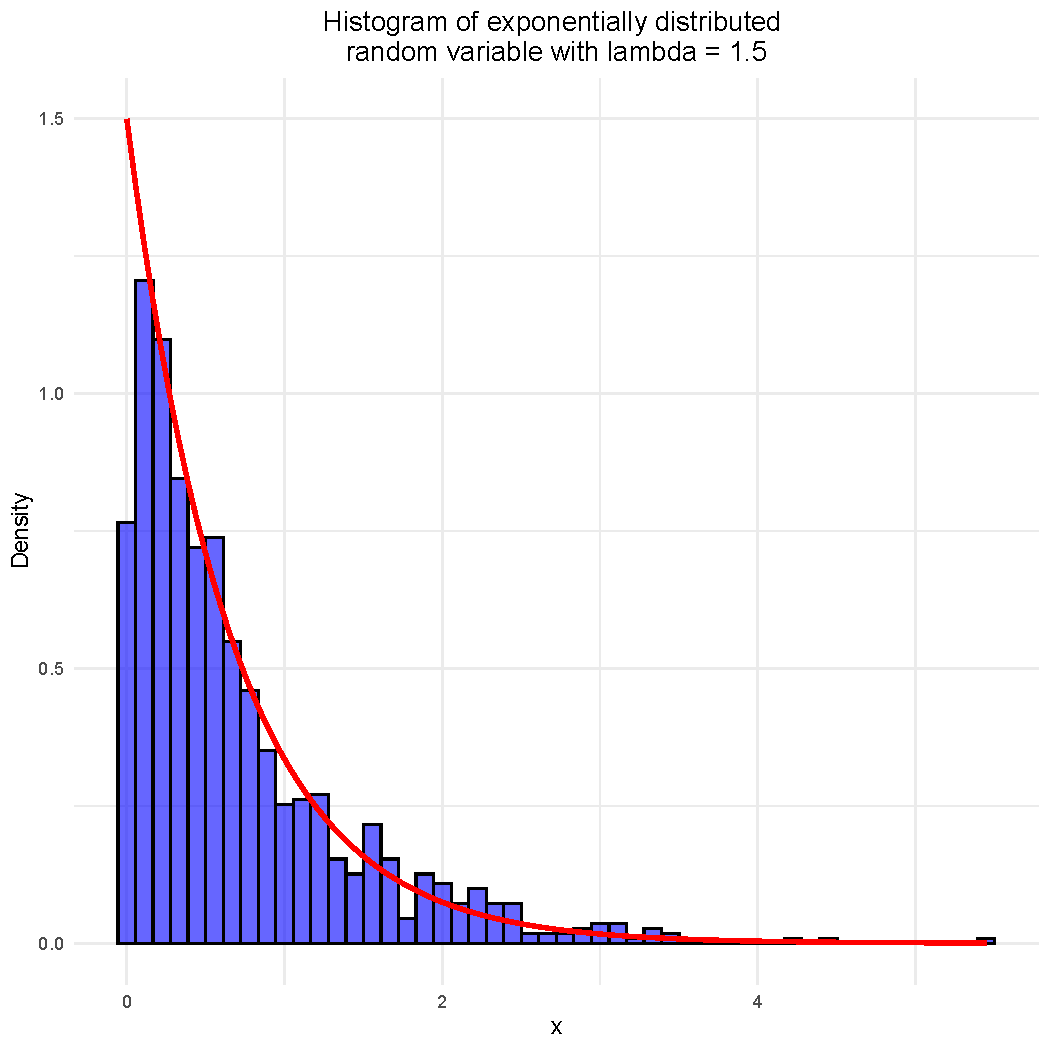
\includegraphics[width=0.7\linewidth]{img/img-1-5-1.jpeg}
	\caption{Exponential distributed random variable; histogram of 1000 generated points and theoretical distribution}
	\label{fig:img-1-6-1}
\end{figure}

\subsubsection{Write down the log-likelihood function for this exponentially distributed random variable.}

For sample $\mathbf{x} = ( x_1, \dots, x_n )^T$ obtained on an exponential distributed random variable $X$, with parameter vector $\mathbf{\theta}=(\lambda)$, the likelihood


\begin{flalign*}
	L(\mathbf{x}, \mathbf{\theta})	&= \prod_{i=1}^{n} f(x_i, \mathbf{\theta}) \\
		&=  \prod_{i=1}^{n} \lambda e^{-\lambda x_i} \\
		&= \lambda^n e^{\sum_{i=1}^n \lambda x_i}
\end{flalign*}

\noindent The log-likelihood is then

$$	
l(\mathbf{x}, \mathbf{\theta}) = n \space \log(\lambda) - \lambda \sum_{i=0}^{n} x_i	
$$

\noindent Taking the derivative with respect to $\lambda$,

$$
\frac{\partial l(\mathbf{x}, \mathbf{\theta}) }{\partial\lambda} =
\frac{n}{\lambda} - \sum_{i=0}^{n} x_i	
$$

\noindent for maximum $\frac{\partial l(\mathbf{x}, \mathbf{\theta}) }{\partial\lambda}$

\begin{flalign*}
	L\frac{\partial l(\mathbf{x}, \mathbf{\theta}) }{\partial\lambda}	&= 0 \\ 
	\frac{n}{\lambda} - \sum_{i=0}^{n} x_i	 &= 0 \\
	\frac{n}{\lambda}  &= \sum_{i=0}^{n} x_i	
\end{flalign*}

\noindent So that

\begin{equation}
	\hat{\lambda} = \frac{n}{\sum_{i=0}^{n} x_i	} = \frac{1}{\overline{x}}
\end{equation}


\subsubsection{Evaluate the log-likelihood function for the generated data as a function of $\lambda$, and plot the resulting log-likelihood function against different values of $\lambda$. Present the plot together with the answers.}


The following listing calculates and plots the log-likelihood values for an exponential distribution with varying $\lambda$ values. The resulting plot can be examined in Figure \ref{fig:img-1-6-2}


\begin{lstlisting}
lambda_values <- seq(0.1, 5, by = 0.01)
log_likelihood_values <- sapply(lambda_values,
function(lambda) LL_exponential(lambda, x))

df <- data.frame(lambda_values, log_likelihood_values)

p <- ggplot(df, 
	aes(x = lambda_values, 
	y = log_likelihood_values)) +
geom_point(
	color = "blue",
	alpha = 0.6) +
	labs(
	title = "Log-Likelihood with varying
 lambda values",
	x = "Lambda",
	y = "Log-Likelihood") +
theme_bw()

quartz()
print(p)
\end{lstlisting}

\begin{figure}[H]
	\centering
	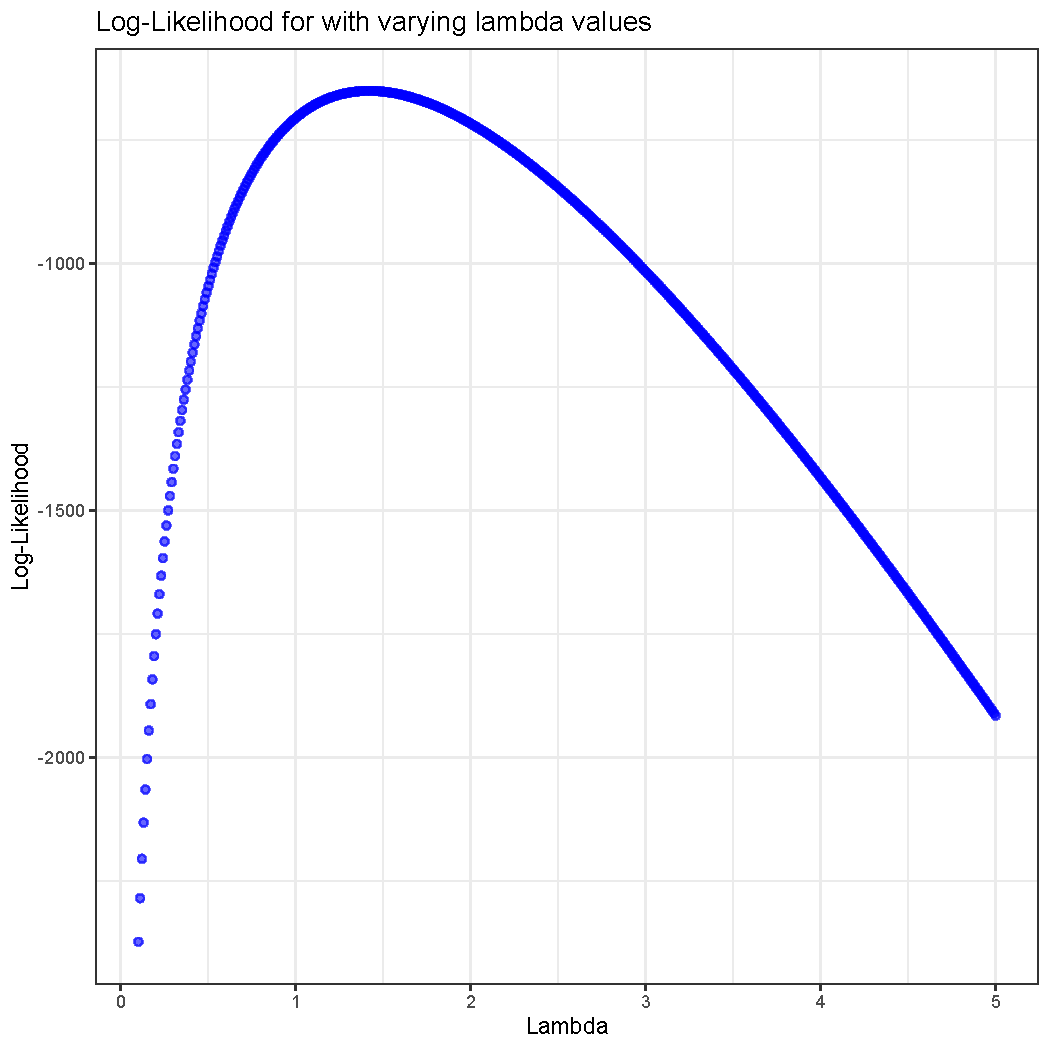
\includegraphics[width=0.7\linewidth]{img/img-1-6-2.jpeg}
	\caption{Log-likelihood plot for an exponential distribution with varying $\lambda$}
	\label{fig:img-1-6-2}
\end{figure}


\subsubsection{Using the plot or otherwise, which estimate for $\lambda$ is the MLE? Give a reason for your answer.}

As we have seen in the previous question, the maximum likelihood estimation is the value for which the derivative of the log-likelihood with respect to lambda is zero, that is the peak of the curve shown in Figure \ref*{fig:img-1-6-2}. This can be easily calculated using the code below. The value obtained for $\hat{\lambda}$ was \textbf{1.43}.

\begin{lstlisting}
max_ll <- max(log_likelihood_values)
max_lambda <- lambda_values[log_likelihood_values == max_ll]
print(glue("Lambda value for maximum log-likelihood is {max_lambda}"))
\end{lstlisting}

%------------------------------------------------------------------------------------------------------------------------
%------------------------------------------------------------------------------------------------------------------------

\section{Question 2}

\textbf{Suppose that we wish to estimate the parameters of the model:}

$$
y_i = \beta_0 + \beta_1 x_{i1} + \beta_2 x_{i2} + \beta_3 x_{i3}^3 + \varepsilon_i
$$

\noindent \textbf{given a sample of size $n$}.

\subsection{State the type of estimator that needs to be used in this situation and mention two properties of this estimator.}

The appropriate estimator for the given regression model:

$$
y_i = \beta_0 + \beta_1 x_{i1} + \beta_2 x_{i2} + \beta_3 x_{i3}^3 + \varepsilon_i
$$


is the Ordinary Least Squares Estimator. This estimator is used because it is linear in parameters, even though $x_3^3$introduces a non-linear transformation. In addition, Ordinary Least Squares minimizes the sum of squared residuals to obtain the best fit for the parameters. Properties of the Ordinary Least Squares estimator include:

\begin{itemize}
	\item Unbiasedness. The Ordinary Least Squares estimator is unbiased, meaning its expected value equals the true parameter value; $\mathbb{E}[\hat{\beta}] = \beta$.
	\item Best Linear Unbiased Estimator. Ordinary Least Squares provides the lowest variance among all linear unbiased estimators, making Ordinary Least Squares the most efficient estimator when errors have constant variance (homoscedasticity).
\end{itemize}



\subsection{Derive the equations that need to be solved to obtain the required estimates.}


\noindent For the given model:
$$
y_i = \beta_0 + \beta_1 x_{i1} + \beta_2 x_{i2} + \beta_3 x_{i3}^3 + \varepsilon_i
$$

\noindent The sum os squared residuals will be minimized using ordinary least squares.

$$
S = \sum_{i=1}^{n} (\varepsilon_i = \sum_{i-1}^{n} y_i - \beta_0 - \beta_1 x_{i1} - \beta_2 x_{i2} - \beta_3 x_{i3}^3)
$$

\noindent Our aim is to find $$\arg \max_{\beta_0, \beta_1, \beta_2, \beta_3} S$$ 

\noindent by equating 
$$ 
\frac{\partial S}{\partial \beta_0} = 0, 
\frac{\partial S}{\partial \beta_1} = 0, 
\frac{\partial S}{\partial \beta_2} = 0, 
\frac{\partial S}{\partial \beta_3} = 0
$$

\noindent that is,

\begin{flalign*}
\frac{\partial S}{\partial \beta_0} =& 2 \sum_{i=1}^{n} (\varepsilon_i = \sum_{i-1}^{n} y_i - \beta_0 - \beta_1 x_{i1} - \beta_2 x_{i2} - \beta_3 x_{i3}^3) = 0 \\
\frac{\partial S}{\partial \beta_1} =& \sum_{i=1}^{n} (\varepsilon_i = \sum_{i-1}^{n} y_i - \beta_0 - \beta_1 x_{i1} - \beta_2 x_{i2} - \beta_3 x_{i3}^3) (-x_{i1} )= 0 \\
\frac{\partial S}{\partial \beta_2} =& \sum_{i=1}^{n} (\varepsilon_i = \sum_{i-1}^{n} y_i - \beta_0 - \beta_1 x_{i1} - \beta_2 x_{i2} - \beta_3 x_{i3}^3)(-x_{i2}) = 0 \\
\frac{\partial S}{\partial \beta_3} =& \sum_{i=1}^{n} (\varepsilon_i = \sum_{i-1}^{n} y_i - \beta_0 - \beta_1 x_{i1} - \beta_2 x_{i2} - \beta_3 x_{i3}^3) (-x_{i3}^3) = 0 
\end{flalign*}	

\noindent rearranging,

\begin{flalign*}
	\sum_{i=1}^{n}y_i =& n \beta_0 +\beta_1 \sum_{i=1}^{n} x_{i1} + \beta_2 \sum_{i=1}^{n} x_{i2} + \beta_3 \sum_{i=1}^{n} x_{i_3}^3 \\
	\sum_{i=1}^{n}y_ix_{i1} =& \beta_0 \sum_{i=1}^{n} x_{i1}  +\beta_1 \sum_{i=1}^{n} x_{i1}^2 + \beta_2 \sum_{i=1}^{n} x_{i2}x_{i1} + \beta_3 \sum_{i=1}^{n} x_{i_3}^3x_{i1} \\
	\sum_{i=1}^{n}y_ix_{i2} =& \beta_0 \sum_{i=1}^{n} x_{i2}  +\beta_1 \sum_{i=1}^{n} x_{i1}x_{i2} + \beta_2 \sum_{i=1}^{n} x_{i2}^2 + \beta_3 \sum_{i=1}^{n} x_{i_3}^3x_{i2} \\
	\sum_{i=1}^{n}y_ix_{i_3}^3 =& \beta_0\sum_{i=1}^{n} x_{i_3}^3 +\beta_1 \sum_{i=1}^{n} x_{i1}x_{i_3}^3 + \beta_2 \sum_{i=1}^{n} x_{i2}x_{i_3}^3 + \beta_3 \sum_{i=1}^{n} x_{i_3}^6
\end{flalign*}


\noindent that can be written in matrix form as follows:

\begin{equation}
\label{eqn:2.3-soln}
	\begin{bmatrix}
		\sum_{i=1}^{n}y_i \\
		\sum_{i=1}^{n}y_ix_{i1}\\
		\sum_{i=1}^{n}y_ix_{i2}\\
		\sum_{i=1}^{n}y_ix_{i_3}^3
	\end{bmatrix}
	=
	\begin{bmatrix}
		n  							& \sum_{i=1}^{n} x_{i1} 			& \sum_{i=1}^{n} x_{i2} 			& \sum_{i=1}^{n} x_{i_3}^3 \\
		\sum_{i=1}^{n} x_{i1}  		& \sum_{i=1}^{n} x_{i1}^2 			& \sum_{i=1}^{n} x_{i2}x_{i1}		& \sum_{i=1}^{n} x_{i_3}^3x_{i1} \\
		\sum_{i=1}^{n} x_{i2}  		& \sum_{i=1}^{n} x_{i1}x_{i2} 		& \sum_{i=1}^{n} x_{i2}^2 			& \sum_{i=1}^{n} x_{i_3}^3x_{i2} \\
		\sum_{i=1}^{n} x_{i_3}^3	& \sum_{i=1}^{n} x_{i1}x_{i_3}^3 	& \sum_{i=1}^{n} x_{i2}x_{i_3}^3 	& \sum_{i=1}^{n} x_{i_3}^6
	\end{bmatrix}
	\begin{bmatrix}
		\beta_0\\
		\beta_1\\
		\beta_2\\
		\beta_3\\
	\end{bmatrix}
\end{equation}


\noindent Equation \ref{eqn:2.3-soln} needs to be solved to obtain the required estimates. But let us try to move this a bit further. If we ser the design matrix $\textbf{X}$ as follows:

$$
\textbf{X}
=
\begin{bmatrix}
1	& x_{11}	& x_{12}	& x_{13} \\
1	& x_{21}	& x_{22}	& x_{23} \\
1	& \vdots	& \vdots	& \vdots \\
1	& x_{n1}	& x_{n2}	& x_{n3} \\
\end{bmatrix}
$$

\noindent We can see that

$$
\textbf{X}^T \textbf{X}
=
\begin{bmatrix}
	n  							& \sum_{i=1}^{n} x_{i1} 			& \sum_{i=1}^{n} x_{i2} 			& \sum_{i=1}^{n} x_{i_3}^3 \\
	\sum_{i=1}^{n} x_{i1}  		& \sum_{i=1}^{n} x_{i1}^2 			& \sum_{i=1}^{n} x_{i2}x_{i1}		& \sum_{i=1}^{n} x_{i_3}^3x_{i1} \\
	\sum_{i=1}^{n} x_{i2}  		& \sum_{i=1}^{n} x_{i1}x_{i2} 		& \sum_{i=1}^{n} x_{i2}^2 			& \sum_{i=1}^{n} x_{i_3}^3x_{i2} \\
	\sum_{i=1}^{n} x_{i_3}^3	& \sum_{i=1}^{n} x_{i1}x_{i_3}^3 	& \sum_{i=1}^{n} x_{i2}x_{i_3}^3 	& \sum_{i=1}^{n} x_{i_3}^6
\end{bmatrix}
$$

\noindent and

$$
\textbf{X}^T \textbf{Y}
=
\begin{bmatrix}
	\sum_{i=1}^{n}y_i \\
	\sum_{i=1}^{n}y_ix_{i1}\\
	\sum_{i=1}^{n}y_ix_{i2}\\
	\sum_{i=1}^{n}y_ix_{i_3}^3
\end{bmatrix}
$$

\noindent Therefore Equation \ref{eqn:2.3-soln} can be written as

\begin{equation}
	\mathbf{X}^T \mathbf{Y} = \mathbf{X}^T \mathbf{X} \boldsymbol{\beta}
\end{equation}

\noindent so that

\begin{equation}
	\boldsymbol{\beta} = (\mathbf{X}^T \mathbf{X})^{-1} \mathbf{X}^T \mathbf{Y}
\end{equation}


$\mathbf{X}^T \mathbf{X}$  is known as the Gram matrix and represents the relationships among predictor variables in a regression model. Its inverse, $(\mathbf{X}^T \mathbf{X})^{-1}$, plays a crucial role in calculating the variance and standard errors of the estimated regression coefficients. Specifically, the diagonal elements of $(\mathbf{X}^T \mathbf{X})^{-1}$ are used to compute the standard errors of the estimated coefficients. The standard error of $\hat{\beta}_j$ is given by:

$$
SE(\hat{\beta}_j) = \sqrt{\sigma^2 \cdot \left( (\mathbf{X}^T \mathbf{X})^{-1} \right)_{jj}}
$$

where $\sigma^2$ is the residual variance, and $\left( (\mathbf{X}^T \mathbf{X})^{-1} \right)_{jj}$ is the diagonal element corresponding to $\beta_j$. This formulation ensures that the uncertainty in the coefficient estimates accounts for correlations between predictors, making it a fundamental component in statistical inference for regression models.


\subsection{ Generate or source a dataset for which you would use this type of model and fit the model to the data.  Present a plot of the fitted model to the data.  Comment on the goodness of fit of the model to the data.  The R code used for this question should be presented together with the answers. Proper referencing should be provided in the text if the data is sourced.}

Listing \ref{lst:ols} creates a synthetic dataset for this examples and fits the specified linear model. It can be summarized as follows:

\begin{enumerate}
	\item The predictor variable ranges are first defined. The predictor variables are then generated with random noise to introduce variability, which ensures numerical stability in regression computations.  
	
	\item The regression coefficients are then specified; $\beta_0 = 5$, $\beta_1 = 2.5$, $\beta_2 = -1.2$, $\beta_3 = 0.8$
	
	\item The response variable ($y$) is computed as a linear combination of $x_1$ and $x_2$, along with a cubic transformation of $x_3$ to capture non-linear effects.  
	
	\item Random noise is added to the response variable to simulate measurement error and external variability, forcing the model to account for stochastic influences.  
	
	\item A multiple regression model is then fitted to estimate the relationships between predictors and the response variable while incorporating the cubic transformation of $x_3$ to capture non-linear patterns.  
\end{enumerate}


\begin{figure}[H]
	\captionsetup{type=lstlisting}
	\begin{lstlisting}
set.seed(2023)

library(ggplot2)

# Generate data

number_of_samples <- 1000

limits_x1 <- c(-10, 10)
limits_x2 <- c(-7, 5)
limits_x3 <- c(-3, 8)

x1 <- seq(limits_x1[1], limits_x1[2], length.out = number_of_samples) + rnorm(number_of_samples, mean = 0, sd = 2)  # Add slight randomness
x2 <- seq(limits_x2[1], limits_x2[2], length.out = number_of_samples) + rnorm(number_of_samples, mean = 0, sd = 2)  # Add slight randomness
x3 <- seq(limits_x3[1], limits_x3[2], length.out = number_of_samples) + rnorm(number_of_samples, mean = 0, sd = 2)  # Add slight randomness

beta_0  <- 5
beta_1  <- 2.5
beta_2  <- -1.2
beta_3  <- 0.8

y <- beta_0 + (beta_1 * x1) + (beta_2 * x2) + (beta_3 * x3^3)
error <- rnorm(length(y), mean = 0.1, sd = 10)  # Random noise
y_real <- y + error


model <- lm(y_real ~ x1 + x2 + I(x3^3))
print(summary(model))			
		\end{lstlisting}
	\caption{Data generation and model fitting using Ordinary Least Squares}
	\label{lst:ols}
\end{figure}

The following table lists the \texttt{summary} results that were obtained. Figure \ref{fig:img-2-3-2} shows the actual vs. predicted values for our model. The plot suggests that the model’s predictions are very close to the actual values, meaning it captures most of the variance in the data.


\begin{longtable}{|p{0.4\textwidth}|p{0.6\textwidth}|}
	\hline
	\textbf{Regression Output} & \textbf{Comment} \\
	\hline

	\hline
	\multicolumn{2}{|c|}{\textbf{Call}} \\
	\hline
	\texttt{lm(formula = y\_real ~ x1 + x2 + I(x3\textasciicircum3))} & 
	Specifies a linear regression where $y$ is predicted using $x_1$, $x_2$, and $x_3^3$. The function \texttt{I(x3\textasciicircum3)} ensures $x_3$ is cubed as a transformation. \\
	\hline

	\hline
	\multicolumn{2}{|c|}{\textbf{Residuals}} \\
	\hline
	\texttt{Min = -31.031} & Smallest residual (largest over-prediction). \\
	\hline
	\texttt{1Q = -6.926} & First quartile (25\% of residuals are below this). \\
	\hline
	\texttt{Median = -0.218 }& Median residual, close to zero suggests unbiased predictions. \\
	\hline
	\texttt{3Q = 6.738} & Third quartile (75\% of residuals are below this). \\
	\hline
	\texttt{Max = 33.252} & Largest residual (largest under-prediction). \\
	\hline
	\texttt{residuals plot} (not part of summary but generated subsequently) & \parbox[c]{5cm}{\centering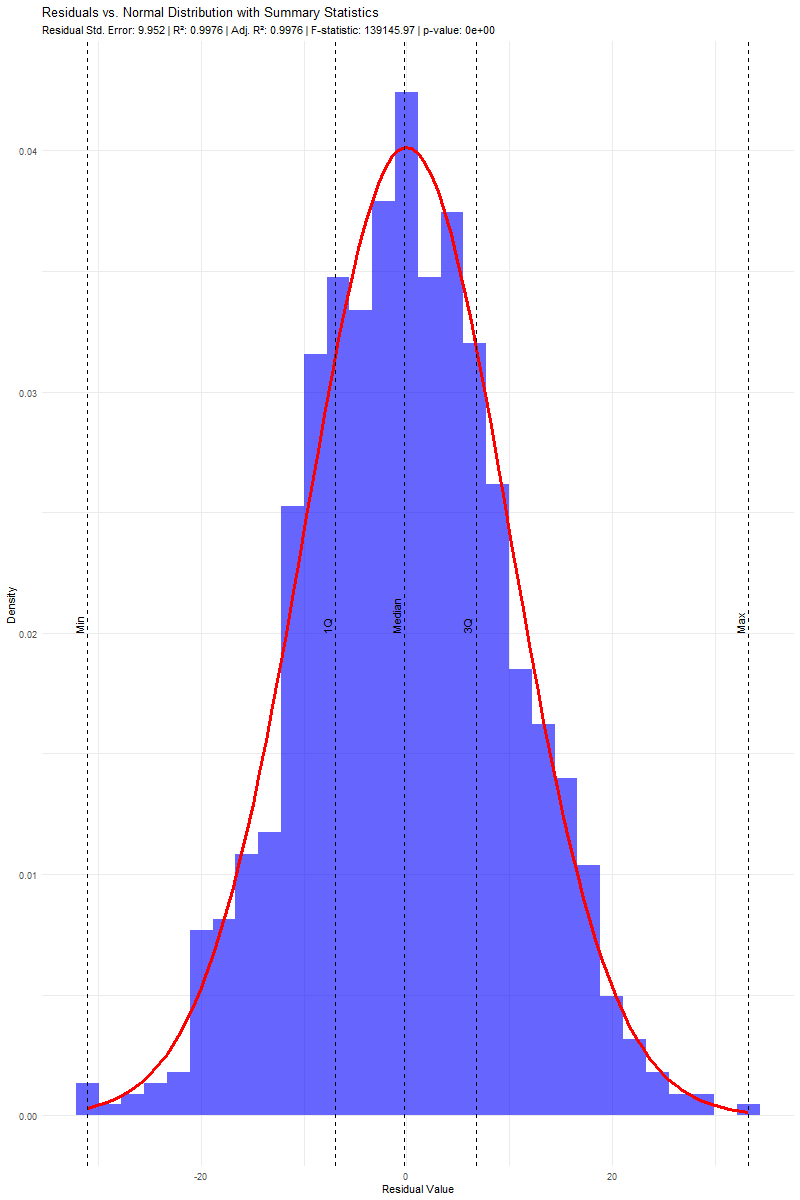
\includegraphics[width=4cm]{img/img-2-3-1}} \\
	\hline

	\hline	
	\multicolumn{2}{|c|}{\textbf{Coefficients}} \\
	\hline
	\texttt{(Intercept)  = 5.44611} & $\hat{\beta_0}$\\
	\hline
	\texttt{x1  = 2.67591} & $\hat{\beta_1}$\\
	\hline
	\texttt{x2 = -1.41965} & $\hat{\beta_2}$\\
	\hline
	\texttt{I(x3\textasciicircum3) = 0.80047} & $\hat{\beta_3}$\\
	\hline

	\hline
	\multicolumn{2}{|c|}{\textbf{Standard Errors (Precision of Estimates)}} \\
	\hline
	\texttt{Intercept SE} = 0.39241 & Standard error for $\beta_0$. Smaller SE suggests a reliable estimate. \\
	\hline
	\texttt{x1 SE} = 0.09603 & Standard error for $\beta_1$. A small SE implies that estimates are stable. \\
	\hline
	\texttt{x2 SE} = 0.13976 & Standard error for $\beta_2$. Suggests moderate precision but check for multicollinearity. \\
	\hline
	\texttt{I(x3\textasciicircum3) SE} = 0.00157 & Very small SE, indicating high precision and a narrow confidence interval. \\
	\hline
	\multicolumn{2}{|c|}{\textbf{t-values (Test Statistic for Significance)}} \\
	\hline
	\texttt{Intercept t-value} = 13.88 & Indicates the intercept is statistically significant. \\
	\hline
	\texttt{x1 t-value} = 27.86 & Strong evidence that $x_1$ affects $y$. Practical significance should also be considered. \\
	\hline
	\texttt{x2 t-value} = -10.16 & Strong evidence that $x_2$ affects $y$. Multicollinearity should be assessed. \\
	\hline
	\texttt{I(x3\textasciicircum3) t-value} = 509.81 & Extremely strong effect of $x_3^3$ on $y$. Consider checking residual plots for outliers. \\
	\hline


	\hline
	\multicolumn{2}{|c|}{\textbf{p-values (Significance Levels)}} \\
	\hline
	\texttt{Intercept p-value < 2e-16} & Highly significant \texttt{(p < 0.001)}. \\
	\hline
	\texttt{x1 p-value < 2e-16} & Highly significant \texttt{(p < 0.001)}. \\
	\hline
	\texttt{x2 p-value < 2e-16} & Highly significant \texttt{(p < 0.001)}. \\
	\hline
	\texttt{I(x3\textasciicircum3) p-value < 2e-16} & Highly significant \texttt{(p < 0.001)}. \\
	\hline

	\hline
	\multicolumn{2}{|c|}{\textbf{Model Fit Statistics}} \\
	\hline
	\texttt{Residual standard error = 9.952} & Measures average prediction error. \\
	\hline
	\texttt{Multiple $R^2 = 0.9976$} & Model explains 99.76\% of the variance in $y$. \\
	\hline
	\texttt{Adjusted $R^2 = 0.9976$} & Adjusted for the number of predictors, still very high. \\
	\hline
	\texttt{F-statistic = $1.391 \times 10^5$} & Tests overall model significance. \\
	\hline
	\texttt{Model p-value < 2.2e-16} & Overall model is highly significant. \\
	\hline
\end{longtable}
	


\begin{figure}[H]
	\centering
	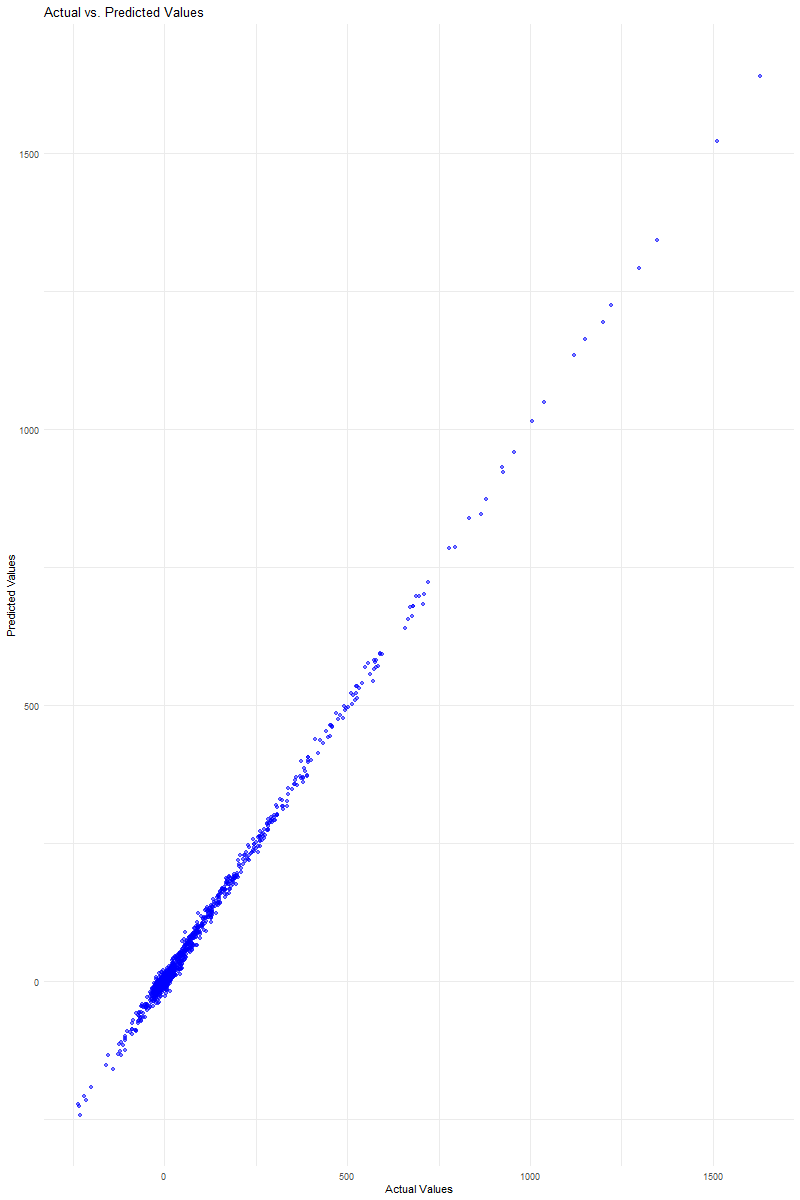
\includegraphics[width=0.7\linewidth]{img/img-2-3-2}
	\caption{Predicted vs. actual values of the response variable}
	\label{fig:img-2-3-2}
\end{figure}




%------------------------------------------------------------------------------------------------------------------------
%------------------------------------------------------------------------------------------------------------------------


\section{Question 3}

Let $x_1, \dots, x_n$ be a random sample selected from a population with a distribution of your choice. [This distribution needs to be different from those used in the lecture notes].

\subsection{Derive the maximum likelihood estimator/s of the parameters of the chosen distribution.}

For this problem we will examine the famous Pareto distribution that is used to describe a wide range of phenomena. The probability density function for this distribution is given by;

$$
f(x; \alpha, x_m) = 
\begin{cases}
\frac{\alpha x_{m}^{\alpha}}{x^{\alpha+1}} & x\ge x_m\\
0 & otherwise
\end{cases}
\text{   for  }\alpha > 0  \quad x_m > 0, 
$$

Where
\begin{itemize}
	\item The shape parameter or tail index $\alpha$ defines thickness of the distribution tail. 
	\item The scale parameter $x_m$ represents the minimum  possible value that random variable $X$ can take in the distribution.
\end{itemize}

\noindent The likelihood function for this distribution;


$$
L(x; \alpha, x_m) = \prod_{i=1}^{n} \frac{\alpha x_{m}^{\alpha}}{x_i^{\alpha+1}}
$$

\noindent then,

\begin{flalign*}
l(x; \alpha, x_m) &= \sum_{i=1}^{n} \log \left(  \frac{\alpha x_{m}^{\alpha}}{x_i^{\alpha+1}} \right)\\
	&= \sum_{i=1}^{n}  \left(  \log (\alpha x_{m}^{\alpha}) - \log(x_i^{\alpha+1}) \right)\\
	&= \sum_{i=1}^{n} \log (\alpha x_{m}^{\alpha}) - \sum_{i=1}^{n} \log(x_i^{\alpha+1}) \\
	&= \sum_{i=1}^{n} \log (\alpha) + \sum_{i=1}^{n} \log (x_{m}^{\alpha}) - \sum_{i=1}^{n} \log(x_i^{\alpha+1}) \\
	&= n \log (\alpha) + n \alpha \log (x_{m}) - (\alpha+1)\sum_{i=1}^{n} \log(x_i) \\
\end{flalign*}


\noindent As the probability density function is only defined for $x_i \ge x_m$, the likelihood is zero iff $x_m \le \min(x_1 \dots x_n)$.
So, the maximum likelihood estimate of $x_m$ is the largest value such that all observed data are $\ge x_m$. This implies:

$$
\widehat{x_m} = \min(x_1 \dots x_n)
$$


\noindent Similarly,

$$
\frac{\partial l(x; \alpha, x_m)}{\partial \alpha} = \frac{n}{\alpha} + n \: \log(x_m) - \sum_{i=1}^{n} \log(x_i)
$$

\noindent for maximum likelihood

\begin{flalign*}
\frac{n}{\alpha} + n \: \log(x_m) - \sum_{i=1}^{n} \log(x_i) &= 0\\
-\frac{n}{\alpha} - n \: \log(x_m) + \sum_{i=1}^{n} \log(x_i) &= 0\\
-\frac{n}{\alpha} - \sum_{i=1}^{n} \log(x_m) + \sum_{i=1}^{n} \log(x_i) &= 0\\
-\frac{n}{\alpha} + \sum_{i=1}^{n} \log \frac{x_i}{x_m} &= 0
\end{flalign*}

\noindent Hence;

$$
\widehat{\alpha} = \frac{n}{\sum_{i=1}^{n} \log \frac{x_i}{x_m}}
$$


\noindent Where  $x_i \ge x_m$ and $\widehat{x_m} = \min(\textbf{x})$, so,


$$
\widehat{\alpha} = \frac{n}{\sum_{i=1}^{n} \log \frac{x_i}{\min(x_1 \dots x_n)}}
$$

\noindent  Hence the maximum likelihood estimators are:

$$
\widehat{x_m} = \min(x_1 \dots x_n), \quad \widehat{\alpha} = \frac{n}{\sum_{i=1}^{n} \log   \frac{x_i}{\min(x_1 \dots x_n)}}
$$


\subsection{Find the Cramer-Rao lower bound for the maximum likelihood estimator/s obtained in Q3i).}

\noindent The likelihood for a single observation
$$
L(x; \alpha, x_m) = \frac{\alpha x_{m}^{\alpha}}{x^{\alpha+1}} ;\quad x\ge x_m
$$

\noindent The log likelihood
$$
l(x; \alpha, x_m) = \log(\alpha) +\alpha \log(x_m) -(\alpha+1) log(x)
$$

\noindent For $x_m$, the score function

$$
\frac{\partial l(x; \alpha, x_m)}{\partial x_m} = \frac{\alpha}{x_m} ;\quad x\ge x_m, x_m>0, \alpha>0
$$

\noindent Taking the second derivative with respect to $x_m$
$$
\frac{\partial^2 l(x; \alpha, x_m)}{\partial x_m^2} = -\frac{\alpha}{x_m^2} ;\quad x\ge x_m, x_m>0, \alpha>0
$$

\noindent The expected value;

$$
E \left[ \frac{\partial^2 l(x; \alpha, x_m)}{\partial x_m^2} \right] = -\frac{\alpha}{x_m^2} ;\quad x\ge x_m, x_m>0, \alpha>0
$$

\noindent Fisher information for n samples,

$$
I_n(x_m) = \frac{n\alpha}{x_m^2};\quad x\ge x_m, x_m>0, \alpha>0
$$

\noindent So CRLB,

$$
Var(\widehat{x_m}) \ge \frac{x_m^2}{n\alpha};\quad x_m>0, \alpha>0
$$

\noindent For $\alpha$, the score function
$$
\frac{\partial l(x; \alpha, x_m)}{\partial \alpha} = \frac{1}{\alpha} + \log(x_m) - \log(x) ;\quad x\ge x_m, x_m>0, \alpha>0
$$

\noindent Taking the second derivative with respect to $\alpha$
$$
\frac{\partial^2 l(x; \alpha, x_m)}{\partial \alpha^2} = -\frac{1}{\alpha^2} ;\quad x\ge x_m, x_m>0, \alpha>0
$$

\noindent The expected value;

$$
E \left[ \frac{\partial^2 l(x; \alpha, x_m)}{\partial \alpha^2} \right]  = -\frac{1}{\alpha^2} ;\quad x\ge x_m, x_m>0, \alpha>0
$$

\noindent Fisher information for n samples,

$$
I_n(\alpha) = \frac{n}{\alpha^2};\quad x\ge x_m, x_m>0, \alpha>0
$$

\noindent So CRLB,

$$
Var(\widehat{\alpha}) \ge \frac{\alpha^2}{n};\quad \alpha>0
$$


\subsection{Does/do the ML estimator/s obtained in Q3i) attain the Cramer-Rao lower bound?  Give a reason for your answer. }

We start this discussion by finding $\mathbb{E}[\widehat{\alpha}]$, where as we have seen
$$
\widehat{\alpha} = \frac{n}{\sum_{i=1}^{n} \log \frac{x_i}{x_m}} \quad, x_m >0
$$
where $\log$ is the natural log, and 
$$
x_i \sim \text{Pareto}(\alpha, x_m)
$$

\noindent We focus on the denominator
$$
S = \sum_{i=1}^{n} \log \frac{x_i}{x_m}
$$

\noindent and understand its distribution so that we can arrive at the estimate of $\mathbb{E}[\widehat{\alpha}]$; and so we start by just understanding the distribution of $ \log \frac{X_i}{x_m}$. If we define

$$
Y = \log \frac{X}{x_m}
$$
so that 
$$
X = x_m e^{Y}
$$

The cumulative distribution function of $Y$ is

\begin{align*}
	F_Y(y) &= \mathbb{P}(Y \leq y) \quad, \forall y \\
			&= \mathbb{P}(\log \frac{X}{x_m} \leq y) \\
			&= \mathbb{P}(\frac{X}{x_m} \leq e^{y}) \\
			&= \mathbb{P}(X \leq x_m e^{y}) \\
\end{align*}

for a Pareto distribution, the cumulative distribution function,
$$
F_X(x) = \mathbb{P}(X\leq x) = 1 - \left( \frac{x_m}{x} \right)^\alpha \quad ,x \ge x_m
$$

So,

\begin{align*}
	F_Y(y) &= \mathbb{P}(X \leq x_m e^{y}) \\
			&= 1 - \left( \frac{x_m}{x} \right)^\alpha \quad ,x \ge x_m \\
			& = 1 - e^{-y\alpha} \quad , \alpha \ge 0
\end{align*}

\noindent differentiation to obtain the probability distribution function,

$$
Y = \log \left(\frac{X}{x_m}\right) \sim \text{Exponential}(\alpha)
$$

\noindent Moving on to $S = \sum_{i=1}^{n} \log \frac{x_i}{x_m}$ where $\log(x_i/x_m)$ are i.i.d and exponential with rate $\alpha$, so $S$ follows a Gamma distribution.

$$
S \sim \text{Gamma}(n, \alpha)
$$

\noindent The p.d.f. for this Gamma distribution is
$$
f_S(s) = \frac{\alpha^n}{\Gamma (n)} s^{n-1} e^{-\alpha s}, \quad s > 0
$$

\noindent To find $\mathbb{E}[\hat{\alpha}]$, since

$$
\hat{\alpha} = \frac{n}{S}
$$

\noindent Then

$$
\mathbb{E}\left[\hat{\alpha}\right] = n \mathbb{E}[\frac{1}{S}]
$$

\noindent Now

\begin{align*}
E \left[\frac{1}{S}\right] &= \int_{0}^{\infty} \frac{1}{S} f(s) ds\\
							&= \int_{0}^{\infty} \frac{1}{S}  \frac{\alpha^n}{\Gamma (n)} S^{n-1} e^{-\alpha s} ds \\
							&= \frac{\alpha^n}{\Gamma (n)} \int_{0}^{\infty} \frac{1}{S} S^{n-1} e^{-\alpha s} ds \\
							&= \frac{\alpha^n}{\Gamma (n)} \int_{0}^{\infty} S^{n-2} e^{-\alpha s} ds \\
\end{align*}

\noindent Since 
$$
\Gamma(n) = \int_{0}^{\infty} S^{n-1} e^{-s} dS \\
$$

\noindent If we let

\begin{align*}
u = \alpha S\\
\text{so that } S=\frac{u}{\alpha}\\
\text{and } ds = \frac{1}{\alpha} du
\end{align*}


\begin{align*}
	\int_{0}^{\infty} S^{n-2} e^{-\alpha s} dS  &= \int_{0}^{\infty} \left(\frac{u}{\alpha} \right)^{n-2} e^{-u}\frac{1}{\alpha} du \\
												&= \frac{1}{\alpha^{n-1}} \int_{0}^{\infty} u^{n-2} e^{-u} du \\
												&= \frac{1}{\alpha^{n-1}} \Gamma(n-1)
\end{align*}

\noindent And therefore, 

\begin{align*}
E \left[\frac{1}{S}\right] &= \frac{\alpha^n}{\Gamma (n)} \frac{1}{\alpha^{n-1}} \Gamma(n-1)\\
							&=  \frac{\alpha\Gamma (n-1)}{\Gamma (n)}\\
							&=  \frac{\alpha\Gamma (n-1)}{(n-1)\Gamma (n-1)}\\
							&=  \frac{\alpha}{(n-1)}
\end{align*}



\noindent Let us also consider,

\begin{align*}
	E \left[\frac{1}{S^2}\right] &= \int_{0}^{\infty} \frac{1}{S^2} f(s) ds\\
	&= \int_{0}^{\infty} \frac{1}{S^2}  \frac{\alpha^n}{\Gamma (n)} S^{n-1} e^{-\alpha s} ds \\
	&= \frac{\alpha^n}{\Gamma (n)} \int_{0}^{\infty} \frac{1}{S^2} S^{n-1} e^{-\alpha s} ds \\
	&= \frac{\alpha^n}{\Gamma (n)} \int_{0}^{\infty} S^{n-3} e^{-\alpha s} ds \\
\end{align*}

\noindent If we let

\begin{align*}
	u = \alpha S\\
	\text{so that } S=\frac{u}{\alpha}\\
	\text{and } ds = \frac{1}{\alpha} du
\end{align*}

\begin{align*}
	\int_{0}^{\infty} S^{n-3} e^{-\alpha s} dS  &= \int_{0}^{\infty} \left(\frac{u}{\alpha} \right)^{n-3} e^{-u} \frac{1}{\alpha} du \\
										&= \frac{1}{\alpha^{n-2}} \int_{0}^{\infty} u^{n-3} e^{-u} du \\
										&= \frac{1}{\alpha^{n-2}} \Gamma(n-2)
\end{align*}


\begin{align*}
	E \left[\frac{1}{S^2}\right] &= \frac{\alpha^n}{\Gamma (n)} \frac{1}{\alpha^{n-2}} \Gamma(n-2)\\
	&=  \frac{\alpha^2\Gamma (n-2)}{\Gamma (n)}\\
	&=  \frac{\alpha^2\Gamma (n-2)}{(n-2)(n-1)\Gamma (n-2)}\\
	&=  \frac{\alpha^2}{(n-2)(n-1)}
\end{align*}



\noindent And therefore, since $\hat{\alpha} = \frac{n}{S}$

$$
\mathbb{E}[\hat{\alpha}] = \frac{n\alpha}{n-1}
$$

\noindent and

$$
\mathbb{E}[\hat{\alpha}^2] = \frac{n^2\alpha^2}{(n-2)(n-1)}
$$

\noindent Now,

\begin{align*}
	\text{Var}(\hat{\alpha}) &= \mathbb{E}[\hat{\alpha}^2] - \mathbb{E}[\hat{\alpha}]^2\\
						&= \frac{n^2\alpha^2}{(n-2)(n-1)} - \frac{n^2\alpha^2}{(n-1)^2}\\
						&= n^2\alpha^2 \left( \frac{(n-1)-(n-2)}{(n-2)(n-1)^2}\right)\\
						&= \frac{n^2\alpha^2}{(n-2)(n-1)^2}\\
\end{align*}


\noindent This variance is greater than the Cramer Rao lower bound as,
$$
\frac{n^2\alpha^2}{(n-2)(n-1)^2}  > \frac{\alpha^2}{n} \quad ,\forall n>2
$$

\noindent We also notice that as $n \rightarrow \infty$, the variance approaches $\frac{\alpha^2}{n}$, and hence $\hat{\alpha}$ becomes asymptotically unbiased.

\bigskip

Let us now consider $\hat{x}_m$, where we have found out that $\hat{x}_m=\min(x_1, \dots , x_n)$, where,\\
$$
x_i \sim \text{Pareto}(\alpha, x_m)
$$

\noindent If $Y = \min(X_1, \dots, X_n)$, the cumulative distribution function,

$$
F_Y(y) = 1 - \left( \frac{x_m}{y} \right)^{n\alpha}, \quad y \ge x_m
$$

\noindent Differentiating to obtain the probability distribution function,

\begin{align*}
	f_Y(y) &= \frac{d}{dy} \left( 1- \frac{x_m^{n\alpha}}{y^{n\alpha}} \right), \quad y \ge x_m\\
			&= -\left( n\alpha \frac{x_m^{n\alpha}}{y^{n\alpha+1}} \right)\\
			&= \frac{n\alpha  x_m^{n\alpha}}{y^{n\alpha+1}} 
\end{align*}

\noindent Now, 


\begin{align*}
	\mathbb{E}[\hat{x}_m] &= \mathbb{E}[Y] \\
					&= \int_{x_m}^{\infty} y ~ \frac{n\alpha  x_m^{n\alpha}}{y^{n\alpha+1}} dy\\
					&= n\alpha  x_m^{n\alpha} \int_{x_m}^{\infty} \frac{1}{y^{n\alpha}} dy \\
					&= n\alpha  x_m^{n\alpha} \left[ \frac{y^{-n\alpha+1}}{-n\alpha+1} \right]_{x_m}^{\infty}\\
	\text{As } \lim_{y \to \infty} y^{-n\alpha+1} = 0\\
					&= n\alpha  x_m^{n\alpha} \left( \frac{-x_m^{-n\alpha+1}}{-n\alpha+1} \right), \quad n\alpha > 1 \\
					&= n\alpha  x_m^{n\alpha} \left( \frac{x_m^{1-n\alpha}}{n\alpha-1} \right)\\
					&=   \frac{n\alpha x_m}{n\alpha-1} \\					
\end{align*}

\noindent As $\mathbb{E}[\hat{x}_m] \ne x_m$, $\hat{x}_m=\min(x_1, \dots , x_n)$ is a biased estimate and does not attain the Cramer Rao lower bound.


\subsection{Is/are the ML estimator/s obtained in Q3i) a sufficient statistic for the population parameter/s?  Give a reason for your answer.}


Let us consider the sufficiency of $\hat{x}_m$. As

$$
f(x_i; x_m)=
\begin{cases}
	\frac{\alpha x_m^\alpha}{x_i^{\alpha+1}}, & x_i \ge x_m, \\
	0, & \text{otherwise}.
\end{cases}
$$

\begin{align*}
	f(x_1, \dots, x_n; x_m) &= \prod_{i=1}^{n} \frac{\alpha x_m^\alpha}{x_i^{\alpha+1}}, \quad x_m \le \min(x_1, \dots, x_n) \\
							&= \alpha^n x_m^{n \alpha} \prod_{i=1}^{n} x_i^{-(\alpha+1)}, \quad x_m \le \min(x_1, \dots, x_n)\\
							&\text{We can rewrite this using an indicator function,}\\
							&= \alpha^n x_m^{n \alpha} \prod_{i=1}^{n} x_i^{-\alpha-1} \cdot \mathbf{1}_{\{x_m \le \min{(x_1, \dots, x_n)}\}}\\
							&= \alpha^n x_m^{n \alpha}  \cdot \mathbf{1}_{\{x_m \le \min{(x_1, \dots, x_n)} \}} \prod_{i=1}^{n} x_i^{-\alpha-1}\\
							&\text{Let } T(x) = \min{(x_1, \dots, x_n)} \\
							&= \left(x_m^{n \alpha}  \cdot \mathbf{1}_{\{x_m \le T(x)\}}\right) \left(\alpha^n \prod_{i=1}^{n} x_i^{-\alpha-1}\right) \\
							&= g(T(x);x_m) h(x)
\end{align*}

\noindent So by Neyman-Fisher $T(x) = \min{(x_1, \dots, x_n)}$ is a sufficient statistic of $x_m$


Considering also the sufficiency of $\hat{\alpha}$


$$
f(x_i; \alpha)= \frac{\alpha x_m^\alpha}{x_i^{\alpha+1}}, \quad x_i \ge x_m
$$


\begin{align*}
	f(x_1, \dots, x_n; \alpha) &= \prod_{i=1}^{n} \frac{\alpha x_m^\alpha}{x_i^{\alpha+1}} \\
								&= \alpha^n x_m^{n \alpha} \prod_{i=1}^{n} x_i^{-\alpha-1} \\
								&= \alpha^n e^{\log(x_m^{n\alpha})} e^{\log(\prod_{i=1}^{n} x_i^{-\alpha-1})}\\
								&= \alpha^n e^{n\alpha \log(x_m)} e^{ (-\alpha-1)\sum_{i=1}^{n} \log(x_i)}\\
								&= \alpha^n e^{n\alpha \log(x_m) + (-\alpha-1)\sum_{i=1}^{n} \log(x_i)}\\
								& \text{Let } T(x) = \sum_{i=1}^{n} \log(x_i) \\
								&= \left(\alpha^n e^{n\alpha \log(x_m) + (-\alpha-1) T(x) }\right)\left(1\right) \\
								&= g(T(x);x_m) h(x)
\end{align*}

\noindent So $\sum_{i=1}^{n} \log(x_i)$ is a sufficient statistic of $\alpha$. Furthermore,

\begin{align*}
	\hat{\alpha} &= \frac{n}{\sum_{i=1}^{n} \log(\frac{x_i}{x_m}) }\\
				 &=  \frac{n}{\sum_{i=1}^{n} \left(\log(x_i) - \log(x_m)\right) }\\
				 &=  \frac{n}{\sum_{i=1}^{n} \log(x_i) - \sum_{i=1}^{n} \log(x_m) }\\
\end{align*}

\noindent Since $T(x)$ is a sufficient statistic for $\alpha$ and $\hat{\alpha}$ is a function of $T(x)$, it follows that $\hat{\alpha}$ is also sufficient for $\alpha$.


\subsection{Why are maximum likelihood estimators considered to be desirable estimators?  Mention one situation where a maximum likelihood estimator might not be optimal.}


Maximum likelihood estimators are considered desirable estimators due to several properties,

\begin{itemize}
	\item \textbf{Consistency}. As the sample size increases, the maximum likelihood estimator converges in probability to the parameter's actual value.
	\item \textbf{Asymptotic Normality}. The distribution of the maximum likelihood estimator approaches a normal distribution centred on the actual parameter value.
	\item \textbf{Asymptotic Efficiency}. Among all consistent and asymptotically normal estimators, the maximum likelihood estimator achieves the lowest possible asymptotic variance; it attains the Cramér-Rao Lower Bound asymptotically.
	\item \textbf{Invariance}. If $\widehat{\theta}$ is the maximum likelihood estimator for $\theta$, then $g(\widehat{\theta})$ is the maximum likelihood estimator for $g(\theta)$.
	\item \textbf{Generality}. Maximum likelihood estimators can be applied to various distributions and likelihood models, even in complex or multivariate settings.
\end{itemize}

Maximum likelihood estimators re not always optimal, particularly in small samples.


In the Pareto($\alpha$, $x_m$) case examined in this question:

The Maximum likelihood estimator for $x_m$ is:
$$
\widehat{x}_m = \min(x_1, \dots, x_n)
$$

Although this is the Maximum likelihood estimator, it is biased, and we showed:
$$
\mathbb{E}[\widehat{x}_m] = \frac{n\alpha}{n\alpha - 1} x_m \neq x_m
$$

Moreover, $\widehat{x}_m$ does not attain the Cramér-Rao lower bound, and its bias persists even in large samples.

This illustrates a situation where the Maximum likelihood estimator does not perform optimally, especially in small samples: it is biased, inefficient, and may not be the best choice if an unbiased or minimum variance estimator is available.


%------------------------------------------------------------------------------------------------------------------------
%------------------------------------------------------------------------------------------------------------------------

\section{Question 4 - Jackknife and bootstrap}

\textbf{Consider 50 observations of bivariate pair $(X,Y)$ in resampling.xlsx. Use the nls command in R to estimate the non-linear regression $Y=\frac{aX}{b+X} + \epsilon$.}

\bigskip

The code in Listing \ref{lst:nls} performs non-linear regression on the dataset. The resulting plots are presented in Figure \ref{fig:img-4-1}. The estimated parameters are $\hat{a} = 14.56$ and $\hat{b} = 7.10$.


\begin{figure}[H]
	\captionsetup{type=lstlisting}
	\begin{lstlisting}
library(openxlsx)
library(ggplot2)

# load file
script_dir <- getwd()
file_path <- file.path(script_dir, "resampling.xlsx")
df <- read.xlsx(file_path, colNames = TRUE)

print(c("number of rows: ", nrow(df)))

# estimate the parameters of the model
init_a <- 1
init_b <- 1

nls_model <- nls(y ~ (a * x) / (b + x),
data = df,
start = list(a = init_a, b = init_b))


estimated_params <- coef(nls_model)
a_hat <- estimated_params["a"]
b_hat <- estimated_params["b"]
cat("Estimated a:", a_hat, "\n")
cat("Estimated b:", b_hat, "\n")

# predict the values of y
df$Predicted <- predict(nls_model)
print(head(df))

# plot the data
p <- ggplot(df, aes(x = x  , y = y)) +
geom_point(color = "blue", alpha = 0.5) +
geom_line(aes(
	y = Predicted),
	color = "red",
	linewidth = 1) +
labs(title = "Nonlinear Regression: Y = (aX) / (b+X)",
x = "X", y = "Y") +
theme_minimal()

print(p)
	\end{lstlisting}
\caption{Non linear regression code in R}
\label{lst:nls}
\end{figure}

\begin{figure}[H]
	\centering
	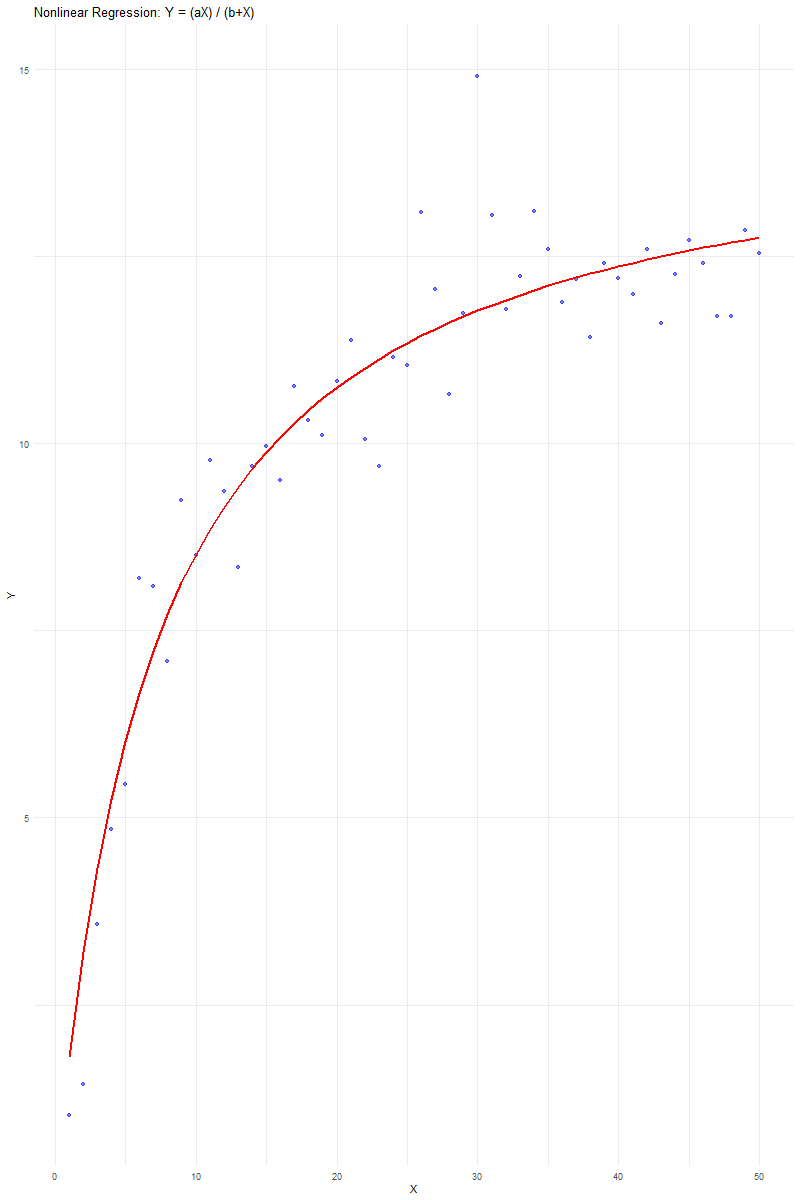
\includegraphics[width=0.7\linewidth]{img/img-4-1}
	\caption{Non-linear regression fit: observed vs. predicted values}
	\label{fig:img-4-1}
\end{figure}


\subsection{Construct a computer code in R to find the Jackknife and Bootstrap estimators of $a$ and $b$. In the case of Jackknife, section randomly the sampling into 5 partitions of size 10. In the case of -
	Bootstrap, generate 1000 samples of size 100 with replacement. }



The code in Listing \ref{lst:jk} executes the following steps on the data to implement Jackknife resampling with non linear regression. The resulting plots are presented in Figure \ref{fig:img-4-1-1}. The estimated parameters are $\hat{a}_{jk} = 14.504$ and $\hat{b}_{jk} = 6.996$. The code executes the following steps to estimate the parameters:

\begin{enumerate}
	\item \textbf{Shuffle the dataset:} We randomly shuffle the data to remove any ordering bias:

	\item \textbf{Divide the data into $m$ Jackknife partitions:} We split the dataset into $m = 5$ partitions, each missing a unique subset of 5 elements.
	
	\item \textbf{Fit the Non-linear Least Squares model for each Jackknife sample:} We fit a non-linear regression model to each Jackknife sample using Non-linear Least Squares to estimate parameters $a$ and $b$. The model is defined as:
	\begin{equation}
		Y = \frac{aX}{b+X}
	\end{equation}
	and is refitted for each sample $S_{-a}$, which excludes partition $P_a$.
	
	\item \textbf{Compute Jackknife bias-corrected estimates:} The Jackknife estimate for each parameter is calculated using the bias correction formula:
	\begin{equation}
		\hat{\theta}_{\text{jack}} = m \hat{\theta} - (m-1) \hat{\theta}_{(-a)}
	\end{equation}
	where:
	\begin{itemize}
		\item $m = 5$ is the number of partitions.
		\item $\hat{\theta}$ is the parameter estimate from the full dataset.
		\item $\hat{\theta}_{(-a)}$ is the parameter estimate from the jackknife sample with partition $a$ removed.
	\end{itemize}
	
	\item \textbf{Compute final Jackknife estimates for $a$ and $b$:} The final Jackknife estimates for $a$ and $b$ are obtained by averaging the bias-corrected values across all jackknife samples:
	\begin{equation}
		\hat{a}_{jk} = \frac{1}{m} \sum_{a=1}^{m} \hat{a}_{\text{jack}, a}, \quad
		\hat{b}_{jk} = \frac{1}{m} \sum_{a=1}^{m} \hat{b}_{\text{jack}, a}
	\end{equation}
\end{enumerate}



\begin{figure}[H]
	\captionsetup{type=lstlisting}
	\begin{lstlisting}
partition_size <- 5

#shuffle the dataframe
set.seed(123)
df_shuf <- df[sample(nrow(df)), ]

# Generate jackknife samples by removing each fold of 5 elements
# lapply applies a function to each element of a list
# my list is from 1:5
# the function will
# for a = 1 remove element 1 to 5 (5*(1-1)+1):(5*1)
# and so on
# note the - sign -- I am removing the elements
# so the return for each a is y without the elements 1 to 5, 6 to 10, etc.
jackknife_samples <- lapply(1:partition_size,
function(a) df_shuf[-((partition_size * (a - 1) + 1):(partition_size * a)), ])

# we have calculated theta_hat_m before
theta_hat_m <- estimated_params

theta_m_a <- function(data) {
	model <- nls(y ~ (a * x) / (b + x),
	data = data,
	start = list(a = theta_hat_m["a"],
	b = theta_hat_m["b"]))
	return(coef(model)) }

# jackknife estimator for each partition
nlsjk <- sapply(jackknife_samples, function(y_a) partition_size * theta_hat_m - (partition_size - 1) * theta_m_a(y_a))

#evaluating the jackknife estimator of the parametrs
jackknife_estimates <- rowMeans(nlsjk)

a_hat_jk <- jackknife_estimates["a"]
b_hat_jk <- jackknife_estimates["b"]

df$predicted_jk <- (a_hat_jk * df$x) / (b_hat_jk + df$x)

# Plot with Jackknife predictions and legend
p_jk <- ggplot(df, aes(x = x, y = y)) +
geom_point(color = "blue", alpha = 0.5, size = 3) +
geom_line(aes(y = Predicted, color = "Full Sample Prediction"),
linewidth = 1, linetype = "dashed") +
geom_line(aes(y = predicted_jk, color = "Jackknife Prediction"),
linewidth = 1) +
labs(title = "Nonlinear Regression: Full Sample vs. Jackknife",
x = "X", y = "Y", color = "Legend") +
theme_minimal() +
scale_color_manual(values = c("Full Sample Prediction" = "red",
"Jackknife Prediction" = "green"))
	\end{lstlisting}
	\caption{Jackknife resampling code in R}
	\label{lst:jk}
\end{figure}

The resulting plot is shown below in Figure \ref{fig:img-4-1-1}


\begin{figure}[H]
	\centering
	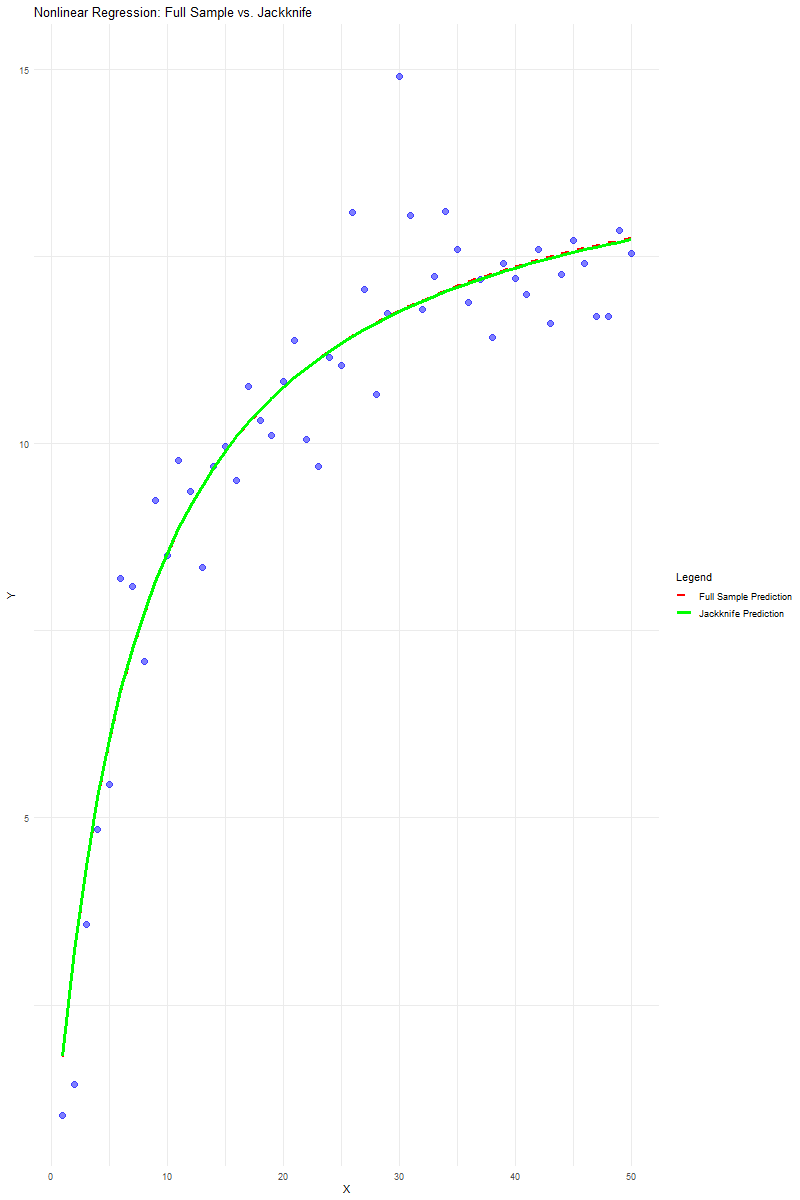
\includegraphics[width=0.7\linewidth]{img/img-4-1-1}
	\caption{Non-linear regression fit: observed vs. predicted values including Jackknife predictions}
	\label{fig:img-4-1-1}
\end{figure}


The code in Listing \ref{lst:bs} executes the following steps on the data to implement Bootstrap resampling with non linear regression. The resulting plots are presented in Figure \ref{fig:img-4-1-2}. The estimated parameters are $\hat{a}_{bs} = 14.566$ and $\hat{b}_{bs} = 7.110$. The code executes the following steps to estimate the parameters:

\begin{itemize}
	\item \textbf{Generate Bootstrap Samples:}  
	WE create 1000 resampled datasets of size 100 by drawing with replacement from the 50 original observations.
	
	\item \textbf{Fit a Non-linear Regression Model:}  
	For each bootstrap sample, we estimate parameters $a$ and $b$ using Non-linear Least Squares with the model.
	
	\item \textbf{Compute Bootstrap Estimates:}  
	The final bootstrap estimates are obtained by averaging the parameter estimates from all bootstrap samples:

	\item \textbf{Predict Values Using Bootstrap Estimates:}  
	Using the estimated parameters $\hat{a}_{\text{bs}}, \hat{b}_{\text{bs}}$, we compute the predicted values:
	\begin{equation}
		\hat{y}_{\text{bs}} = \frac{\hat{a}_{\text{bs}} x}{\hat{b}_{\text{bs}} + x}
	\end{equation}
	
\end{itemize}


\begin{figure}[H]
	\captionsetup{type=lstlisting}
	\begin{lstlisting}
num_samples <- 1000
sample_size <- 100

# 1000 bootstrap samples of size 100 with replacement
bootstrap_samples <- lapply(1:num_samples, function(i) df[sample(nrow(df), sample_size, replace = TRUE), ])

fit_bootstrap_nls <- function(data) {
	model <- nls(y ~ (a * x) / (b + x),
	data = data,
	start = list(a = 1, b = 1))  # Initial guesses
	return(coef(model))
}

# Apply NLS to each bootstrap sample
nlsbs <- lapply(bootstrap_samples, fit_bootstrap_nls)

# Convert list of bootstrap estimates to a matrix
bootstrap_estimates <- do.call(rbind, nlsbs)
colnames(bootstrap_estimates) <- c("a", "b")

# Compute mean estimates for a and b
a_hat_bs <- mean(bootstrap_estimates[, "a"], na.rm = TRUE)
b_hat_bs <- mean(bootstrap_estimates[, "b"], na.rm = TRUE)

# Print results
cat("Bootstrap Estimated a:", a_hat_bs, "\n")
cat("Bootstrap Estimated b:", b_hat_bs, "\n")


df$predicted_bs <- (a_hat_bs * df$x) / (b_hat_bs + df$x)


# Plot with Jackknife predictions and legend
p_bs <- ggplot(df, aes(x = x, y = y)) +
geom_point(color = "blue", alpha = 0.5, size = 3) +
geom_line(aes(y = Predicted, color = "Full Sample Prediction"),
linewidth = 1, linetype = "dashed") +
geom_line(aes(y = predicted_jk, color = "Jackknife Prediction"),
linewidth = 1) +
geom_line(aes(y = predicted_bs, color = "Bootstrap Prediction"),
linewidth = 1) +
labs(title = "Nonlinear Regression: Full Sample vs. Jackknife vs. Bootstrap",
x = "X", y = "Y", color = "Legend") +
theme_minimal() +
scale_color_manual(values = c("Full Sample Prediction" = "red",
"Jackknife Prediction" = "green",
"Bootstrap Prediction" = "blue"))
	\end{lstlisting}
	\caption{Bootstrap resampling code in R}
	\label{lst:bs}
\end{figure}


\begin{figure}[H]
	\centering
	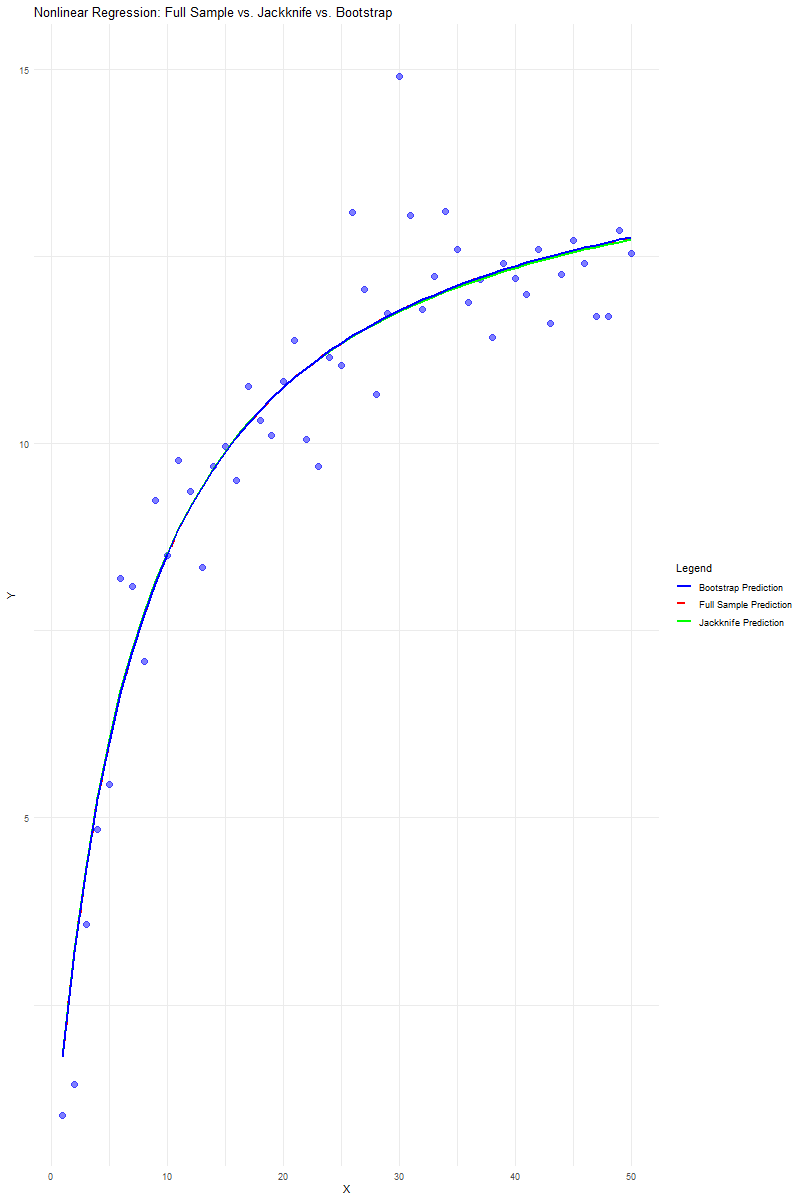
\includegraphics[width=0.7\linewidth]{img/img-4-1-2}
	\caption{Non-linear regression fit: observed vs. predicted values including Jackknife and Bootstrap predictions}
	\label{fig:img-4-1-2}
\end{figure}

\subsection{For the Jackknife estimator, find a 95\% confidence interval using the normal distribution and the t-distribution. For the Bootstrap estimator, find a 95\% normal, t and empirical confidence intervals.}

%To estimate the uncertainty in our parameter estimates, we compute 95\% confidence intervals using the following:
%
%\begin{enumerate}
%	\item \textbf{Compute the standard error (SE):}  
%	\begin{equation}
%		SE = \sqrt{\frac{c}{n} \sum_{i=1}^{n} (\hat{\theta}_{i} - \hat{\theta})^2}
%	\end{equation}
%	where:
%	\begin{itemize}
%		\item $\hat{\theta}_{i}$ is the estimate from the $i$-th resample.
%		\item $\hat{\theta}$ is the mean of all estimates.
%		\item $n$ is the number of resamples: 
%		\begin{itemize}
%			\item number of partitions for Jackknife
%			\item number of resamples for Bootstrap
%		\end{itemize}
%		\item $c$ is a correction factor:
%		\begin{itemize}
%			\item For Jackknife: $c = (m-1)/m$ as bias correction is necessary
%			\item For Bootstrap: $c = 1$  as no correction needed
%		\end{itemize}
%	\end{itemize}
%	
%	\item \textbf{Compute the 95\% confidence interval using the Normal Distribution:}
%	\begin{equation}
%		CI_{\text{normal}} = \hat{\theta} \pm Z_{0.975} \cdot SE
%	\end{equation}
%	where $Z_{0.975} = 1.96$ for a 95\% confidence level.
%	
%	\item \textbf{Compute the 95\% confidence interval using the t-distribution:}
%	\begin{equation}
%		CI_{\text{t}} = \hat{\theta} \pm t_{0.975, df} \cdot SE
%	\end{equation}
%	where:
%	\begin{itemize}
%		\item For Jackknife: $df = m - 1$
%		\item For Bootstrap: $df = B - 1$
%	\end{itemize}
%	
%	\item \textbf{Compute the 95\% confidence interval using the Empirical (Percentile) Method (Bootstrap only):}
%	\begin{equation}
%		CI_{\text{empirical}} = \left[ Q_{0.025}, Q_{0.975} \right]
%	\end{equation}
%	where $Q_{0.025}$ and $Q_{0.975}$ are the 2.5th and 97.5th percentiles of the bootstrap estimates.
%\end{enumerate}
%
%\bigskip

\noindent The following results were obtained for the Jackknife resampling method:

%\begin{itemize}
%	\item 95\% conf. interval for a using normal distribution: [ 14.14397 , 14.86412 ]
%	\item 95\% conf. interval for b using normal distribution: [ 6.356596 , 7.635241 ]
%	\item 95\% conf. interval for a using t-distribution: [ 13.99397 , 15.01412 ]
%	\item 95\% conf. interval for b using t-distribution: [ 6.090267 , 7.90157 ]
%\end{itemize}
%
%
%\noindent The following results were obtained for the Bootstrap resampling method:
%
%\begin{itemize}
%	\item conf. interval for a using normal distribution: [ 14.07722 , 15.05515 ]
%	\item conf. interval for b using normal distribution: [ 6.111358 , 8.109172 ]
%	\item conf. interval for a using t-distribution: [ 14.07663 , 15.05575 ]
%	\item conf. interval for b using t-distribution: [ 6.110146 , 8.110384 ]
%	\item conf. interval for a using empirical distribution: [ 14.08458 , 15.08578 ]
%	\item conf. interval for b using empirical distribution: [ 6.132766 , 8.113393 ]
%\end{itemize}

\begin{table}[h]
	\centering
	\begin{tabular}{|c|c|c|}
		\hline
		\textbf{Method} & \textbf{Confidence Interval for $a$} & \textbf{Confidence Interval for $b$} \\
		\hline
		\multicolumn{3}{|c|}{\textbf{Jackknife Resampling}} \\
		\hline
		Normal Distribution & \texttt{[14.14397, 14.86412]} & \texttt{[6.356596, 7.63524]} \\
		t-Distribution & \texttt{[13.99397, 15.01412]} & \texttt{[6.090267, 7.90157]} \\
		\hline
		\multicolumn{3}{|c|}{\textbf{Bootstrap Resampling}} \\
		\hline
		Normal Distribution & \texttt{[14.07722, 15.05515]} & \texttt{[6.111358, 8.109172]} \\
		t-Distribution & \texttt{[14.07663, 15.05575]} & \texttt{[6.110146, 8.110384]} \\
		Empirical Distribution & \texttt{[14.08458, 15.08578]} & \texttt{[6.132766, 8.113393]} \\
		\hline
	\end{tabular}
	\caption{Confidence Intervals for Parameters $a$ and $b$ Using Jackknife and Bootstrap Methods}
	\label{tab:ci_results}
\end{table}

%------------------------------------------------------------------------------------------------------------------------
%------------------------------------------------------------------------------------------------------------------------


\section{Question 5 – The EM Algorithm }

Consider a univariate $K$-Gaussian mixture model with probability density function:

$$
f(x) = \sum_{l=1}^{K} \pi_l \phi(x, \mu_l, \sigma_l)
$$

\noindent such that $\sum_{l=1}^{K} \pi_l = 1$ and $\pi_l > 0$ for all $l$, and where $\phi(x, \mu, \sigma)$ is the Gaussian density function. The EM algorithm for this works as follows:

\begin{enumerate}
	\item Initialise $\mu_1^{(0)}, \dots, \mu_K^{(0)}, \sigma_1^{(0)}, \dots, \sigma_K^{(0)}, \pi_1^{(0)}, \dots, \pi_K^{(0)}$.
	
	\item Let 
	$$
	\gamma_n^{(j,k)} = \frac{\pi_k \phi(x_n | \mu_k^{(j-1)}, \sigma_k^{(j-1)})}{\sum_{i=1}^{K} \pi_i \phi(x_n | \mu_i^{(j-1)}, \sigma_i^{(j-1)})}.
	$$
	
	\item Let
	$$
	\mu_k^{(J)} = \frac{1}{N_k} \sum_{n=1}^{N} \gamma_n^{(j,k)} x_n, 
	$$
	$$
	\sigma_k^{(J)} = \sqrt{\frac{1}{N_k} \sum_{n=1}^{N} \gamma_n^{(j,k)} (x_n - \mu_k^{(J)})^2},
	$$
	and 
	$$
	\pi_k^{(J)} = \frac{N_{jk}}{N},
	$$
	where
	$$
	N_{jk} = \sum_{n=1}^{N} \gamma_n^{(j,k)}.
	$$
\end{enumerate}



\subsection{Simulate 1000 readings from a mixture Gaussian distribution with 3 or more Gaussians.}

The following function generalizes the code provided in the question so that an arbitrary number of samples are generated from any number of Gaussian distributions. The function also lists the number of samples selected from each Gaussian to ensure that acceptable proportions were attained for each sample and plots a distribution of the data and plots of the Gaussians.

\begin{figure}[H]
	\captionsetup{type=lstlisting}
	\begin{lstlisting}
library(ggplot2)

generate_samples <- function(
mixing_coefficients,
means,
standard_deviations,
number_of_samples = 1000) {
	
	# should check that lengths are equal
	
	data <- c()
	choices_count <- rep(0, length(mixing_coefficients))
	
	# select one of the gaussian distributions according
	# to the mixing coefficients
	choices <- sample(
	x = seq_along(mixing_coefficients),
	size = number_of_samples,
	prob = mixing_coefficients,
	replace = TRUE)
	
	# let us see that the number of selections make sense
	for (i in 1:number_of_samples){
		choices_count[choices[i]] <- choices_count[choices[i]] + 1
	}
	print(choices_count)
	
	# for each selection, sample from the gaussian
	data <- c(
	data,
	rnorm(
	n = number_of_samples,
	mean = means[choices],
	sd = standard_deviations[choices]))
	
	# plot histogram and gaussian curves
	df <- data.frame(data)
	
	p <- ggplot(df, aes(x = data)) +
	geom_histogram(
	aes(y = ..density..),
	bins = 30,
	fill = "blue",
	alpha = 0.6) +
	stat_function(fun = function(x) {
		Reduce(`+`, lapply(1:length(means), function(i) {
			dnorm(
			x = x,
			mean = means[i],
			sd = standard_deviations[i]) * mixing_coefficients[i]
		}))
	}, color = "red") +
	labs(title = "Histogram of Mixture of Gaussians",
	x = "Value",
	y = "Density") +
	theme_bw()
	
	print(p)
}
	\end{lstlisting}
	\caption{Gaussian mixture sample generation code in R}
	\label{lst:gausmix}
\end{figure}

\noindent Data from the mixed Gaussian distributions was subsequently generated using the parameters below. The plot that was obtained as a result of this process is shown in Figure \ref{fig:img-5-1}

\begin{table}[h]
	\centering
	\renewcommand{\arraystretch}{1.2} % Adjust row height
	\begin{tabular}{|c|c|c|}
		\hline
		$\pi_1 = 0.2$ & $\mu_1 = 6$  & $\sigma_1 = 2.0$  \\
		\hline
		$\pi_2 = 0.5$ & $\mu_2 = 0$  & $\sigma_2 = 1.0$  \\
		\hline
		$\pi_3 = 0.3$ & $\mu_3 = -7$ & $\sigma_3 = 1.5$  \\
		\hline
	\end{tabular}
\end{table}

\begin{figure}[H]
	\captionsetup{type=lstlisting}
	\begin{lstlisting}
mixing_coefficients <- c(0.2, 0.5, 0.3)
means <- c(6, 0, -7)
standard_deviations <- c(2, 1, 1.5)

generate_samples(mixing_coefficients, means, standard_deviations)			
		\end{lstlisting}
	\caption{Generation of data for this question}
	\label{lst:gem-gausmix}
\end{figure}

\begin{figure}[H]
	\centering
	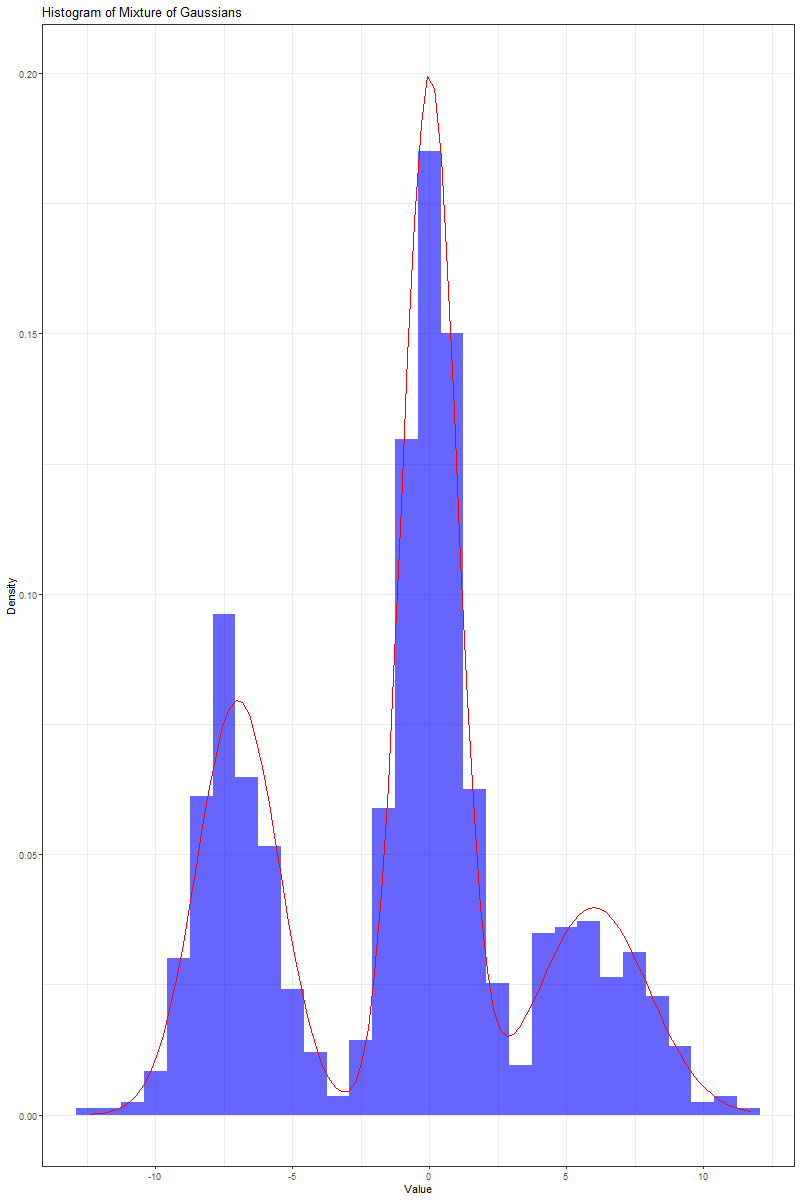
\includegraphics[width=0.5\linewidth]{img/img-5-1}
	\caption{Distribution of generated data}
	\label{fig:img-5-1}
\end{figure}


\subsection{Determine initial values $\mu_1^{(0)}, \dots, \mu_K^{(0)}, \sigma_1^{(0)}, \dots, \sigma_K^{(0)}, \pi_1^{(0)}, \dots, \pi_K^{(0)}$ 	using a K-means clustering approach or otherwise.
}

The function in Listing \ref{lst:kmeans} is a custom implementation of a k-means algorithm to initialize parameters($\mu^{(0)}$, $\sigma^{(0)}$, and $\pi^{(0)}$) for a Gaussian mixture model. Its salient features are the following:
\begin{itemize}
	\item After the initial centroids are randomly selected, the k-means algorithm iteratively assigns the data point to the closest centroid based on the absolute distance. The cluster centroids are then updated as the means of the points assigned to each cluster until the change in centroids is small or the threshold number of iterations is reached.
	\item The means of each centroid is, as we have discussed above, the centroid of each cluster.
	\item the standard deviation is calculated as follows
	$$
	\sigma_j =
	\begin{cases}
		\sqrt{\frac{1}{n_j} \sum_{x_i \in C_j} (x_i - \mu_j)^2}, & \text{if } n_j > 0 \\
		0, & \text{otherwise}
	\end{cases}
	$$
	Where:
	\begin{itemize}
		\item $\sigma_j$ is the standard deviation for cluster $j$,
		\item $C_j$ is the set of points in cluster $j$,
		\item $n_j$ is the number of points in cluster $j$,
		\item $x_i$ are the individual data points in cluster $j$,
		\item $\mu_j$ is the centroid (mean) of cluster $j$,
	\end{itemize}
	
	\item The initial values for the mixing coefficients of the Gaussian Mixture Model are computed as:
	
	$$
	\pi_j =
	\begin{cases}
		\frac{n_j}{N}, & \text{if } n_j > 0 \\
		0, & \text{otherwise}
	\end{cases}
	$$
	
	Where:
	\begin{itemize}
		\item $\pi_j$ is the mixing coefficient for cluster $j$,
		\item $n_j$ is the number of data points in cluster $j$,
		\item $N$ is the total number of data points in the dataset,
	\end{itemize}
	
\end{itemize}


\begin{figure}[H]
	\captionsetup{type=lstlisting}
	\begin{lstlisting}
initial_values_knn <- function(data, k = 3) {
	set.seed(42)  # For reproducibility
	
	# Randomly select k initial centroids
	centroids <- sample(x = data, size = k, replace = FALSE)
	
	# Initialize empty clusters
	clusters <- vector(mode = "list", length = k)
	
	for (iteration in 1:100) {
		# Reset clusters
		clusters <- vector(mode = "list", length = k)
		
		# Assign each data point to the closest centroid
		for (item in data) {
			distances <- abs(item - centroids)
			closest_centroid <- which.min(distances)
			clusters[[closest_centroid]] <- c(clusters[[closest_centroid]], item)
		}
		
		# Compute new centroids
		new_centroids <- sapply(1:k, function(i) {
			if (length(clusters[[i]]) > 0) {
				mean(clusters[[i]])
			} else {
				centroids[i]  # Keep old centroid if no points are assigned
			}
		})
		
		# Check for convergence
		if (max(abs(new_centroids - centroids)) < 0.0001) {
			break
		}
		
		centroids <- new_centroids
	}
	
	# Compute standard deviations
	clusters_standard_devs <- sapply(1:k, function(cluster_idx) {
		if (length(clusters[[cluster_idx]]) > 0) {
			sqrt(sum((clusters[[cluster_idx]] - centroids[cluster_idx])^2) / length(clusters[[cluster_idx]]))
		} else {
			0
		}
	})
	
	# Compute mixing coefficients for each cluster
	mixing_coefficients <- sapply(1:k, function(cluster_idx) {
		length(clusters[[cluster_idx]]) / length(data)
	})
	
	return(list(
	centroids = centroids,
	standard_devs = clusters_standard_devs,
	mixing_coefficients = mixing_coefficients))
}
		
		\end{lstlisting}
	\caption{k-means algorithm to compute the initial values of the mixed Gaussian model parameters}
	\label{lst:kmeans}
\end{figure}

The results obtained from this function are as follows:

\bigskip

\begin{table}[h]
	\centering
	\renewcommand{\arraystretch}{1.2} % Adjust row height
	\begin{tabular}{|c|c|c|}
		\hline
		$\pi_1 = 0.179$ & $\mu_1 = 6.353$  & $\sigma_1 = 1.685$  \\
		\hline
		$\pi_2 = 0.545$ & $\mu_2 = 0.104$  & $\sigma_2 = 1.107$  \\
		\hline
		$\pi_3 = 0.276$ & $\mu_3 = -6.942$ & $\sigma_3 = 1.508$  \\
		\hline
	\end{tabular}
	\caption{Estimated parameters for the initial values of Gaussian mixture model}
	\label{tab:gmm_parameters}
\end{table}

\subsection{Run the EM algorithm for a number of iterations. Print 
	$\mu_1^{(j)}, \dots, \mu_k^{(j)}, \sigma_1^{(j)}, \dots, \sigma_k^{(j)}, \pi_1^{(j)}, \dots, \pi_k^{(j)}$ 
	for each iteration, and also the log-likelihood, which is given by:
	$
	\sum_{n=1}^{N} \ln \left( \sum_{l=1}^{K} \phi(x_i | \mu_l^{(j)}, \sigma_l^{(j)}) \right).
	$
	Determine when to stop the EM algorithm, either via a maximum number of iterations or through a convergence criterion. However, ensure that the EM algorithm has converged. Plot the trajectory of the estimates and the likelihood by iteration to illustrate this.
}


We start by examining the code created to execute this question, which is presented below in four listings.

\begin{itemize}
	\item Listing \ref{lst:em-est} contains the estimation step code that computes the responsibility of each Gaussian component for each data point as:
	
	$$
	\gamma_{n,k} = \frac{\pi_k \phi(x_n | \mu_k, \sigma_k)}{\sum_{j=1}^{K} \pi_j \phi(x_n | \mu_j, \sigma_j)}
	$$
	
	Where:
	\begin{itemize}
		\item $\gamma_{n,k}$ is the responsibility of Gaussian $k$ for data point $x_n$.
		\item $\pi_k$ is the mixing coefficient for Gaussian $k$.
		\item $\phi(x_n | \mu_k, \sigma_k)$ is the Gaussian probability density function:
		$$
		\phi(x_n | \mu_k, \sigma_k) = \frac{1}{\sigma_k \sqrt{2\pi}} \exp \left( -\frac{(x_n - \mu_k)^2}{2\sigma_k^2} \right).
		$$
	\end{itemize}	
	
	
	\item Listing \ref{lst:em-max} illustrates the maximization step of the EM algorithm that updates the parameters as follows:
	
	\begin{itemize}
		\item We update the mixing coefficients to calculate the proportion of data points that belong to a given Gaussian distribution:
		$$
		\pi_k^{(j)} = \frac{N_k^{(j)}}{N}
		$$
		Where:
		$$
		N_k^{(j)} = \sum_{n=1}^{N} \gamma_{n,k}^{(j)}
		$$
		Is the total responsibility weight assigned to Gaussian $k$?
		
		\item We update the means to compute the weighted mean of the data points assigned to each Gaussian:
		$$
		\mu_k^{(j)} = \frac{\sum_{n=1}^{N} \gamma_{n,k}^{(j)} x_n}{N_k^{(j)}}
		$$
		
		\item We update the standard deviations to calculate the spread of the data points around the updated mean for each Gaussian:
		
		$$
		\sigma_k^{(j)} = \sqrt{\frac{\sum_{n=1}^{N} \gamma_{n,k}^{(j)} (x_n - \mu_k^{(j)})^2}{N_k^{(j)}}}
		$$
	\end{itemize}
	
	
	\item We then calculate the log-likelihood function for our Gaussian mixture model using the code in Listing \ref{lst:em-ll} using the suggested formulation:
	
	$$
	\mathcal{L} = \sum_{n=1}^{N} \ln \left( \sum_{k=1}^{K} \pi_k \phi(x_n | \mu_k, \sigma_k) \right)
	$$
	
	Where:
	\begin{itemize}
		\item $\mathcal{L}$ is the log-likelihood of the data.
		\item $K$ is the number of Gaussian components.
		\item $N$ is the number of data points.
		\item $\pi_k$ is the mixing coefficient for Gaussian $k$.
		\item $\phi(x_n | \mu_k, \sigma_k)$ is the Gaussian probability density function:
		$$
		\phi(x_n | \mu_k, \sigma_k) = \frac{1}{\sigma_k \sqrt{2\pi}} \exp \left( -\frac{(x_n - \mu_k)^2}{2\sigma_k^2} \right)
		$$
	\end{itemize}
	
	\item Listing \ref{lst:em-exec} shows the execution of the EM algorithm, starting from the generation of data to the estimation of the initial values and ending with the actual estimates using the EM algorithm. We notice that EM is allowed a maximum of execution 100 steps, but optimization will stop if the change in log-likelihood is smaller than $10^{-5}$.
	
	

\end{itemize}




\begin{figure}[H]
	\captionsetup{type=lstlisting}
	\begin{lstlisting}
expectation_step <- function(data, means, standard_deviations, mixing_coefficients) {
	
	number_of_gaussians <- length(mixing_coefficients)
	
	# Initialize gamma matrix
	gamma <- matrix(0, nrow = length(data), ncol = number_of_gaussians)
	
	# Calculate denominator (total probability for each data point)
	den_total <- 0
	for (k in 1:number_of_gaussians) {
		den_total <- den_total + mixing_coefficients[k] * dnorm(data, mean = means[k], sd = standard_deviations[k])
	}
	
	# Calculate numerator and compute gamma
	for (k in 1:number_of_gaussians) {
		gamma[, k] <- (mixing_coefficients[k] * dnorm(data, mean = means[k], sd = standard_deviations[k])) / den_total
	}
	
	return(gamma)
}			
		\end{lstlisting}
	\caption{Estimation step code in R}
	\label{lst:em-est}
\end{figure}


\begin{figure}[H]
	\captionsetup{type=lstlisting}
	\begin{lstlisting}

maximization_step <- function(data, gamma, means, standard_deviations, mixing_coefficients) {
	
	no_gaussians <- length(mixing_coefficients)
	m <- length(data)
	
	# Compute cluster responsibilities
	m_c <- colSums(gamma)  # Sum of responsibilities for each Gaussian
	
	# Compute new mixing coefficients
	new_mixing_coefficients <- m_c / m
	
	# Initialize new means and standard deviations
	new_means <- numeric(no_gaussians)
	new_standard_deviations <- numeric(no_gaussians)
	
	# Compute new means and standard deviations for each Gaussian
	for (k in 1:no_gaussians) {
		new_means[k] <- sum(gamma[, k] * data) / m_c[k]
		new_standard_deviations[k] <- sqrt(sum(gamma[, k] * (data - means[k])^2) / m_c[k])
	}
	
	return(list(
	means = new_means,
	standard_devs = new_standard_deviations,
	mixing_coefficients = new_mixing_coefficients
	))
}

	\end{lstlisting}
	\caption{Maximization step code in R}
	\label{lst:em-max}
\end{figure}

\begin{figure}[H]
	\captionsetup{type=lstlisting}
	\begin{lstlisting}
log_likelihood <- function(data, means, standard_deviations, mixing_coefficients) {
	
	number_of_gaussians <- length(mixing_coefficients)
	
	# Initialize likelihood matrix
	likelihood <- matrix(0, nrow = length(data), ncol = number_of_gaussians)
	
	# Compute likelihood for each Gaussian component
	for (k in 1:number_of_gaussians) {
		likelihood[, k] <- mixing_coefficients[k] * dnorm(data, mean = means[k], sd = standard_deviations[k])
	}
	
	# Compute the log-likelihood
	log_likelihood_value <- sum(log(rowSums(likelihood)))
	
	return(log_likelihood_value)
}
			
		\end{lstlisting}
	\caption{Log-likelihood code in R}
	\label{lst:em-ll}
\end{figure}

\begin{figure}[H]
	\captionsetup{type=lstlisting}
	\begin{lstlisting}
mixing_coefficients <- c(0.2, 0.5, 0.3)
means <- c(6, 0, -7)
standard_deviations <- c(2, 1, 1.5)

# generate the data
data <- generate_samples(mixing_coefficients, means, standard_deviations)

# initial values
kmeans_ret <- initial_values_kmeans(data)

centroids <- kmeans_ret$centroids
standard_devs <- kmeans_ret$standard_devs
mixing_coefficients <- kmeans_ret$mixing_coefficients

print("initial values")
print(centroids)
print(standard_devs)
print(mixing_coefficients)

log_likelihoods <- c()
for (i in 1:100) {
	gamma <- expectation_step(data, centroids, standard_devs, mixing_coefficients)
	
	max_ret <- maximization_step(data, gamma, centroids, standard_devs, mixing_coefficients)
	
	centroids <- max_ret$means
	standard_devs <- max_ret$standard_devs
	mixing_coefficients <- max_ret$mixing_coefficients 
	
	ll <- log_likelihood(data, means, standard_devs, mixing_coefficients)
	
	log_likelihoods <- c(log_likelihoods, ll)
	
	if (i>2 &&  abs(ll - log_likelihoods[i-1]) < 1e-5) {
		print("converged")
		break
	}
	# form string
	iteration_result_str <- paste( "iteration: ", i)
	for (j in 1:length(centroids)) {
		iteration_result_str <- paste(iteration_result_str, " c",j,": ", format(centroids[j],3))
		iteration_result_str <- paste(iteration_result_str, " s",j,": ", format(standard_devs[j],3))
		iteration_result_str <- paste(iteration_result_str, " m",j,": ", format(mixing_coefficients[j],3))
	}
	print(iteration_result_str)
}			
		\end{lstlisting}
	\caption{Execution code for this question}
\label{lst:em-exec}
\end{figure}


\noindent The parameters obtained after each iteration are shown in Table \ref{tab:gmm_iterations_3dp}. The algorithm converged after 28 iterations. A plot of the log likelihood at each iteration can be observed in Figure \ref{fig:img-5-3}


\begin{table}[H]
	\centering
	\resizebox{0.9\textwidth}{!}{
	\begin{tabular}{|c|c|c|c|c|c|c|c|c|c|c|}
		\hline
		Step & $\pi_1$ & $\sigma_1$ & $\mu_1$ & $\pi_2$ & $\sigma_2$ & $\mu_2$ & $\pi_3$ & $\sigma_3$ & $\mu_3$ & $\mathcal{L}$ \\
		\hline
		1  & 6.259  & 1.780  & 0.183  & 0.088  & 1.101  & 0.541  & -6.936  & 1.519  & 0.276  & -2666.447 \\
		2  & 6.208  & 1.824  & 0.186  & 0.078  & 1.090  & 0.538  & -6.935  & 1.520  & 0.276  & -2665.715 \\
		3  & 6.176  & 1.850  & 0.187  & 0.071  & 1.084  & 0.537  & -6.935  & 1.521  & 0.276  & -2665.371 \\
		4  & 6.155  & 1.868  & 0.188  & 0.067  & 1.079  & 0.536  & -6.934  & 1.521  & 0.276  & -2665.192 \\
		5  & 6.142  & 1.880  & 0.189  & 0.065  & 1.077  & 0.535  & -6.934  & 1.521  & 0.276  & -2665.092 \\
		6  & 6.132  & 1.888  & 0.189  & 0.063  & 1.075  & 0.534  & -6.934  & 1.522  & 0.276  & -2665.033 \\
		7  & 6.126  & 1.893  & 0.189  & 0.062  & 1.074  & 0.534  & -6.934  & 1.522  & 0.276  & -2664.996 \\
		8  & 6.122  & 1.897  & 0.190  & 0.061  & 1.073  & 0.534  & -6.934  & 1.522  & 0.276  & -2664.973 \\
		9  & 6.119  & 1.900  & 0.190  & 0.061  & 1.073  & 0.534  & -6.934  & 1.522  & 0.276  & -2664.958 \\
		10 & 6.117  & 1.901  & 0.190  & 0.061  & 1.072  & 0.534  & -6.934  & 1.522  & 0.276  & -2664.947 \\
		11 & 6.115  & 1.903  & 0.190  & 0.060  & 1.072  & 0.534  & -6.934  & 1.522  & 0.276  & -2664.941 \\
		12 & 6.114  & 1.903  & 0.190  & 0.060  & 1.072  & 0.534  & -6.934  & 1.522  & 0.276  & -2664.936 \\
		13 & 6.114  & 1.904  & 0.190  & 0.060  & 1.072  & 0.534  & -6.934  & 1.522  & 0.276  & -2664.933 \\
		14 & 6.113  & 1.904  & 0.190  & 0.060  & 1.072  & 0.534  & -6.934  & 1.522  & 0.276  & -2664.931 \\
		15 & 6.113  & 1.905  & 0.190  & 0.060  & 1.072  & 0.534  & -6.934  & 1.522  & 0.276  & -2664.929 \\
		16 & 6.113  & 1.905  & 0.190  & 0.060  & 1.072  & 0.534  & -6.934  & 1.522  & 0.276  & -2664.928 \\
		17 & 6.113  & 1.905  & 0.190  & 0.060  & 1.072  & 0.534  & -6.934  & 1.522  & 0.276  & -2664.928 \\
		18 & 6.113  & 1.905  & 0.190  & 0.060  & 1.072  & 0.534  & -6.934  & 1.522  & 0.276  & -2664.927 \\
		19 & 6.112  & 1.905  & 0.190  & 0.060  & 1.072  & 0.534  & -6.934  & 1.522  & 0.276  & -2664.927 \\
		20 & 6.112  & 1.905  & 0.190  & 0.060  & 1.072  & 0.534  & -6.934  & 1.522  & 0.276  & -2664.927 \\
		21 & 6.112  & 1.905  & 0.190  & 0.060  & 1.072  & 0.534  & -6.934  & 1.522  & 0.276  & -2664.926 \\
		22 & 6.112  & 1.905  & 0.190  & 0.060  & 1.072  & 0.534  & -6.934  & 1.522  & 0.276  & -2664.926 \\
		23 & 6.112  & 1.905  & 0.190  & 0.060  & 1.072  & 0.534  & -6.934  & 1.522  & 0.276  & -2664.926 \\
		24 & 6.112  & 1.905  & 0.190  & 0.060  & 1.072  & 0.534  & -6.934  & 1.522  & 0.276  & -2664.926 \\
		25 & 6.112  & 1.905  & 0.190  & 0.060  & 1.072  & 0.534  & -6.934  & 1.522  & 0.276  & -2664.926 \\
		26 & 6.112  & 1.905  & 0.190  & 0.060  & 1.072  & 0.534  & -6.934  & 1.522  & 0.276  & -2664.926 \\
		27 & 6.112  & 1.905  & 0.190  & 0.060  & 1.072  & 0.534  & -6.934  & 1.522  & 0.276  & -2664.926 \\
		28 & 6.112  & 1.905  & 0.190  & 0.060  & 1.072  & 0.534  & -6.934  & 1.522  & 0.276  & -2664.926 \\
		\hline
	\end{tabular}
	}
	\caption{EM iterations results table}
	\label{tab:gmm_iterations_3dp}
\end{table}

\begin{figure}[H]
	\centering
	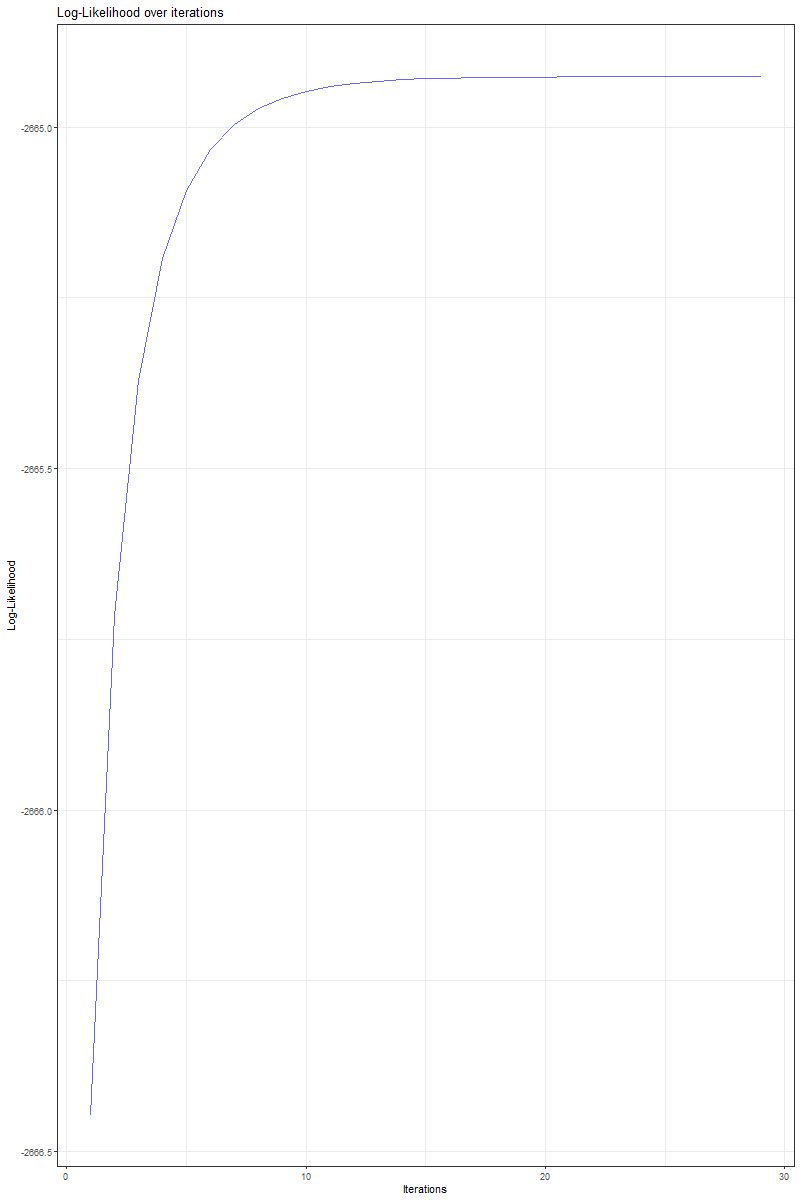
\includegraphics[width=0.7\linewidth]{img/img-5-3}
	\caption{Log-likelihood vs iterations for the execution of the EM algorithm until convergence}
	\label{fig:img-5-3}
\end{figure}

\subsection{Give the final estimated $\mu_k$'s, $\sigma_k$'s and $\pi_k$'s. How do these compare with the coefficients you chose in the simulation?
}


The final estimated values compared to the chosen ones are listed in Table \ref{tab:gmm_chosen_vs_estimated_full}. The estimated values are very close to the initially chosen values, confirming that the initial assumptions were reasonable. The final log-likelihood value of -2664.926 indicates that the EM algorithm successfully converged to a stable solution. The minor parameter adjustments demonstrate that the algorithm effectively fine-tuned the initial estimates based on the data. The estimated values align closely with the assumed mixture structure, validating the underlying data distribution. Minor shifts in mixing coefficients, means, and standard deviations suggest that while the clusters generally adhered to the expected patterns, some exhibited slightly different densities than initially assumed. The successful convergence of the model indicates that the algorithm reached a local maximum of the likelihood function, further confirming the robustness of the estimation process.

\begin{table}[H]
	\centering
	\renewcommand{\arraystretch}{1.2}
	\begin{tabular}{|c|c|c|c|}
		\hline
		Distribution & Parameter & Chosen Value & Estimated Value \\
		\hline
		\multirow{3}{*}{Distribution 1} & $\pi_1$ & 0.200000 & 0.1901318 \\
		& $\mu_1$ & 6.000000 & 6.112331 \\
		& $\sigma_1$ & 2.000000 & 1.905292 \\
		\hline
		\multirow{3}{*}{Distribution 2} & $\pi_2$ & 0.500000 & 0.5335142 \\
		& $\mu_2$ & 0.000000 & 0.05972212 \\
		& $\sigma_2$ & 1.000000 & 1.071750 \\
		\hline
		\multirow{3}{*}{Distribution 3} & $\pi_3$ & 0.300000 & 0.276354 \\
		& $\mu_3$ & -7.000000 & -6.933639 \\
		& $\sigma_3$ & 1.500000 & 1.521854 \\
		\hline
	\end{tabular}
	\caption{Chosen vs. estimated parameters}
	\label{tab:gmm_chosen_vs_estimated_full}
\end{table}



\bibliography{references}
\bibliographystyle{plain}

\end{document}

%\begin{figure}[H]
%	\captionsetup{type=lstlisting}
%	\begin{lstlisting}
%		
%	\end{lstlisting}
%	\caption{Jackknife resampling code in R}
%	\label{lst:jk}
%\end{figure}
%
